%==============================================================================
% Distilling RL Manipulation Policies into Lightweight Supervised Models
% IEEE conference paper (IEEEtran). Compiles on Overleaf / TeXLive (IEEEtran is
% standard). Figures live in images/. \TBD / \figplaceholder remain defined as
% helpers for future placeholders; the current draft has none outstanding.
%==============================================================================
\documentclass[conference]{IEEEtran}
\IEEEoverridecommandlockouts

\usepackage{cite}
\usepackage{amsmath,amssymb,amsfonts}
\usepackage{graphicx}
\usepackage{tikz}
\usetikzlibrary{positioning,arrows.meta,shapes.geometric,fit,backgrounds,calc}
\usepackage{booktabs}
\usepackage{subcaption}
\usepackage{xcolor}
\usepackage{url}
\usepackage[hidelinks]{hyperref}

\graphicspath{{images/}}

% --- placeholder helpers: visible markers for values/figures to fill later ----
\newcommand{\TBD}[1]{\textcolor{red}{\textbf{[TBD: #1]}}}
\newcommand{\figplaceholder}[2]{% #1 = width fraction, #2 = caption-ish hint
  \fbox{\parbox[c][3.2cm][c]{#1\linewidth}{\centering\color{red}\small
  [FIGURE PLACEHOLDER]\\#2\\ \emph{drop generated PNG into images/ and
  replace this box with \textbackslash includegraphics}}}}

\begin{document}

\title{Distilling Reinforcement-Learning Manipulation Policies into Lightweight
Supervised Models Across Robot Morphologies}

\author{
\IEEEauthorblockN{Satyam Singh}
\IEEEauthorblockA{\textit{Dept. of Mechanical Engineering} \\
\textit{MANIT Bhopal}\\
Bhopal, India \\
24216061103}
\and
\IEEEauthorblockN{Jitendra Adhikari}
\IEEEauthorblockA{\textit{CPDSM} \\
\textit{MANIT Bhopal}\\
Bhopal, India}
\and
\IEEEauthorblockN{Emon Barua}
\IEEEauthorblockA{\textit{Dept. of Mechanical Engineering} \\
\textit{MANIT Bhopal}\\
Bhopal, India}
}

\maketitle

%------------------------------------------------------------------------------
\begin{abstract}
Deep reinforcement learning (RL) can learn implicit inverse-kinematics policies
for robotic manipulation without analytical models, but the resulting neural
policies are comparatively opaque and carry a runtime and memory footprint that
is unattractive for resource-constrained deployment in small and medium
enterprises. We investigate whether such policies can be \emph{distilled} into
classical supervised-learning models that are smaller, faster, and easier to
inspect. Using a morphology-agnostic Proximal Policy Optimization (PPO) teacher
trained on a contact-rich non-prehensile pushing task across five manipulators
(custom 3-, 4-, 5-, and 6-DoF arms and a 7-DoF Franka Panda), we generate
successful-trajectory datasets and engineer a compact kinematic feature set that
maps each state to the \emph{change} in the normalized joint command. Four
students---Linear Regression (LR), a Support Vector Machine (SVM), a Random
Forest (RF), and XGBoost---are trained per morphology and redeployed as
closed-loop controllers. We compare them on imitation fidelity ($R^2$),
closed-loop task success, model footprint, and per-step inference latency. In
closed-loop control the random forest is the most robust student across
morphologies and consistently surpasses the teacher on the redundant 7-DoF arm:
across two teacher checkpoints of differing competence and three re-trainings
each, the deterministic RF student beats its teacher in every run. A greedy
re-evaluation exposes the mechanism: the PPO teacher's success on this arm is
largely an artifact of its test-time exploration noise---taking the mean action,
as one would at deployment, collapses it to near zero---whereas the deterministic
student retains its success. On hard, poorly-converged morphologies distillation
therefore does not merely compress the policy but \emph{recovers a deployable
controller the teacher does not itself possess}; on easier arms, whose teachers
are genuinely competent, the one-shot students instead trail them. The linear and
boosted students are competitive on some morphologies but inconsistent. The distilled linear student is orders of magnitude smaller than
the teacher network and runs faster than its forward pass, whereas the random
forest attains its accuracy at a far heavier memory and latency cost. The
results map a clear accuracy--efficiency trade-off for deploying distilled
manipulation policies.
\end{abstract}

\begin{IEEEkeywords}
policy distillation, reinforcement learning, robotic manipulation, inverse
kinematics, model compression, Proximal Policy Optimization
\end{IEEEkeywords}

%==============================================================================
\section{Introduction}
%==============================================================================
Flexible manufacturing and the growth of Micro, Small, and Medium Enterprises
(MSMEs) demand robots that can be repurposed quickly across heterogeneous arm
morphologies \cite{kober}. The classical route to manipulation---analytical
inverse kinematics (IK)---sits awkwardly with this demand: it presumes an
accurate kinematic model, degenerates near singularities, and must be re-derived
whenever a robot's structure or degrees-of-freedom (DoF) change. Deep
reinforcement learning (RL) sidesteps these constraints by learning a direct
state-to-action mapping from interaction, acting as an \emph{implicit},
model-free IK solver \cite{lobbezoo_survey, shahid}.

A trained deep policy, however, is not free to deploy. Its actor is a neural
network evaluated at every control step, its parameters are opaque to inspection,
and shipping a deep-learning runtime onto the low-cost edge controllers common in
MSME automation is cumbersome. This motivates the question at the centre of this
work: \emph{once a competent RL policy has been learned, can its behaviour be
compressed into a model small, fast, and inspectable enough for constrained
deployment, without any further learning in the loop?}

We study this through knowledge distillation, which transfers the behaviour of a
capable ``teacher'' to a simpler ``student'' \cite{hinton, rusu}. A
morphology-agnostic PPO teacher \cite{schulman} is trained once per arm on a
contact-rich, non-prehensile pushing task; its successful rollouts are recorded
and four classical supervised models---Linear Regression (LR), a Support Vector
Machine (SVM), a Random Forest (RF) \cite{breiman}, and XGBoost
\cite{xgboost}---are fit to reproduce its commands. Rather than the absolute
command, each student predicts the \emph{change} in the normalized joint target,
which we integrate online into a closed-loop controller and evaluate directly in
simulation across five morphologies (3--7~DoF).

Treating the students as controllers---not merely as offline regressors---surfaces
three findings that organize the paper. First, the choice of student is a sharp
accuracy--efficiency trade-off: the random forest is the most reliable controller
across morphologies but by far the heaviest, while the linear student is orders of
magnitude smaller and faster yet inconsistent. Second, one-step imitation fidelity
($R^2$) does \emph{not} predict closed-loop success---a model can minimize
per-step error yet still drift over a full episode. Third, and most striking, on
the redundant 7-DoF arm the teacher's own apparent success is largely an artefact
of its test-time exploration noise: evaluated greedily, as one would at
deployment, it nearly vanishes, yet the deterministic random-forest student,
distilled from the teacher's few successful rollouts, retains its competence.
There, distillation is not mere compression but \emph{recovers a deployable
controller the teacher does not itself possess}.

Our contributions are:
\begin{itemize}
  \item A reproducible RL\,$\rightarrow$\,classical-ML distillation pipeline for
        robotic manipulation that operates uniformly across five morphologies
        (3--7~DoF) using a single configuration-driven framework.
  \item A compact kinematic feature representation and a delta-action target
        formulation that turns teacher rollouts into a supervised regression
        problem, together with a deployable closed-loop inference wrapper.
  \item A systematic comparison of LR, SVM, RF, and XGBoost students on
        imitation fidelity, closed-loop task success, model footprint, and
        per-step latency, exposing a sharp accuracy--efficiency trade-off and
        showing that one-step imitation fidelity does not reliably predict
        closed-loop control performance.
  \item The observation, supported by greedy (deterministic) re-evaluation, that
        on the hard 7-DoF arm the PPO teacher's success is largely
        \emph{exploration-noise-borrowed}---it collapses under greedy
        evaluation---whereas the deterministic random-forest student retains it,
        so distillation can \emph{recover a deployable controller the teacher
        does not itself possess}; on easier arms, whose teachers are genuinely
        competent, the one-shot students instead trail them.
\end{itemize}

%==============================================================================
\section{Related Work}
%==============================================================================
\subsection{RL for manipulation and implicit IK}
For a manipulator with joint vector $\theta\in\mathbb{R}^n$ and forward
kinematics $x=f(\theta)$, analytical IK seeks $\theta=f^{-1}(x)$, which is
ill-posed for redundant arms ($n>m$) and unstable near singularities. Numerical
Jacobian-pseudoinverse methods are foundational but brittle and require manual
re-derivation per morphology \cite{kober}. Deep RL instead learns a policy
$\pi_\phi(a\mid s)$ mapping observations to joint commands, sidestepping explicit
Jacobians \cite{lobbezoo_survey, shahid, elguea}. Our teacher follows this
implicit-IK paradigm; the present paper concerns what to do after such a
policy is learned.

\subsection{Policy and knowledge distillation}
Hinton \emph{et al.} \cite{hinton} introduced distillation as training a compact
student to match a larger teacher; Rusu \emph{et al.} \cite{rusu} extended this
to RL policies, showing that student networks can match or exceed teacher
performance while being smaller. Most policy-distillation work keeps the student
a neural network. We instead distill into \emph{non-neural} models---linear,
kernel, and tree ensembles---to maximize interpretability and deployability, and
we evaluate the students in closed loop rather than only by offline accuracy.

\subsection{Lightweight models for control and edge deployment}
Tree ensembles \cite{breiman, xgboost} and linear models are attractive on
constrained hardware due to small footprints and deterministic, low-latency
inference. Their use as \emph{distillation targets} for a continuous-control RL
policy across a family of morphologies, with an explicit footprint/latency
analysis, is the gap this paper addresses.

%==============================================================================
\section{Background: Multi-Morphology PPO Teacher}
%==============================================================================
The teacher is produced by a morphology-agnostic framework; we summarize only the
parts needed to understand the distillation pipeline.

\subsection{Morphology-agnostic architecture}
A command-line entry point and a centralized \texttt{config.py} expose the
kinematic parameters (joint names and limits) of each robot, while mass, inertia,
friction, and damping are parsed from Simulation Description Format (SDF) models
in Ignition Gazebo. Switching the active robot resizes the policy's input and
output layers automatically; the learning code is unchanged. Five morphologies
are supported (Table~\ref{tab:configs}, Fig.~\ref{fig:envs}).
Fig.~\ref{fig:framework} maps the resulting configuration-driven control flow:
a single entry point branches on the chosen morphology, reward, mode, learning
algorithm, and---at deployment---the policy type, so that training a teacher and
evaluating either that teacher or any distilled student are alternative paths
through one framework.

\begin{table}[t]
\centering
\caption{Robot configurations used for training the teacher.}
\label{tab:configs}
\begin{tabular}{lcc}
\toprule
\textbf{Robot} & \textbf{Active joints} & \textbf{Action dim.} \\
\midrule
3-DoF custom    & joint1--3        & 3 \\
4-DoF custom    & joint1--4        & 4 \\
5-DoF custom    & joint1--5        & 5 \\
6-DoF custom    & joint1--6        & 6 \\
7-DoF Panda     & panda\_joint1--7 & 7 \\
\bottomrule
\end{tabular}
\end{table}

\begin{figure}[t]
\centering
\begin{subfigure}[b]{0.32\columnwidth}
  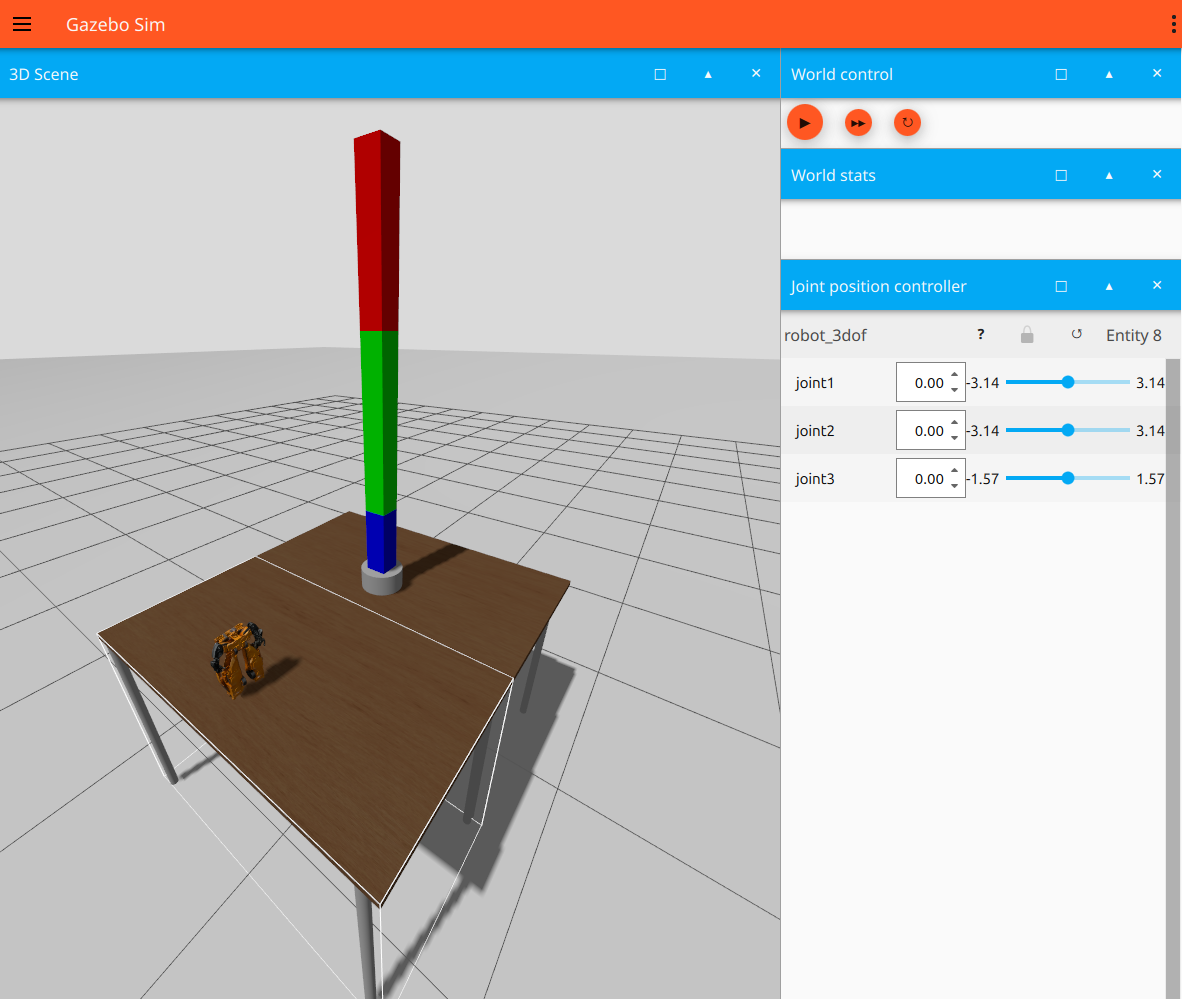
\includegraphics[width=\textwidth]{3DOF.png}\caption{3-DoF}
\end{subfigure}\hfill
\begin{subfigure}[b]{0.32\columnwidth}
  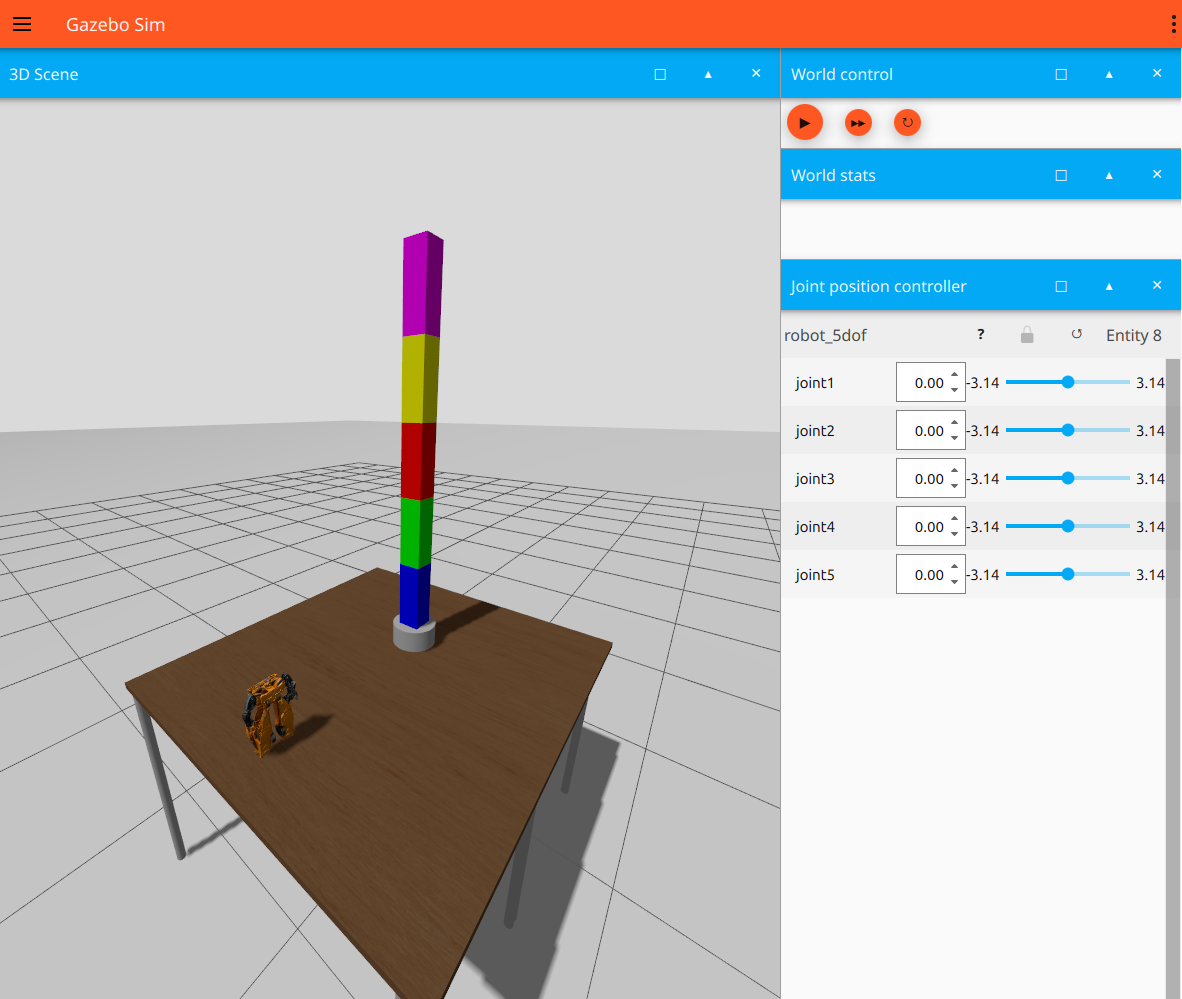
\includegraphics[width=\textwidth]{5DOF.png}\caption{5-DoF}
\end{subfigure}\hfill
\begin{subfigure}[b]{0.32\columnwidth}
  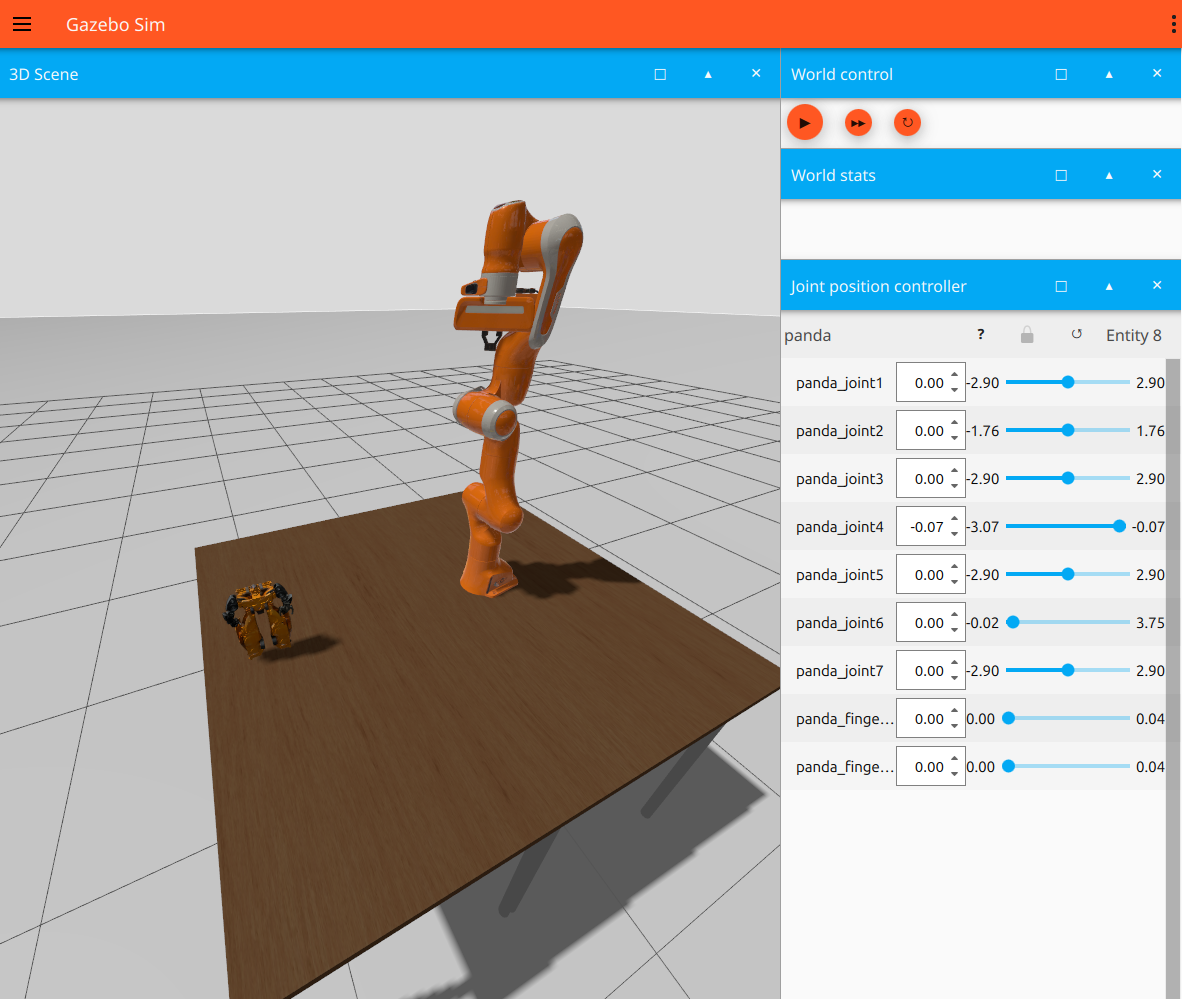
\includegraphics[width=\textwidth]{Panda.png}\caption{7-DoF Panda}
\end{subfigure}
\caption{Representative simulated morphologies in Ignition Gazebo.}
\label{fig:envs}
\end{figure}

\begin{figure*}[t]
\centering
\resizebox{\textwidth}{!}{%
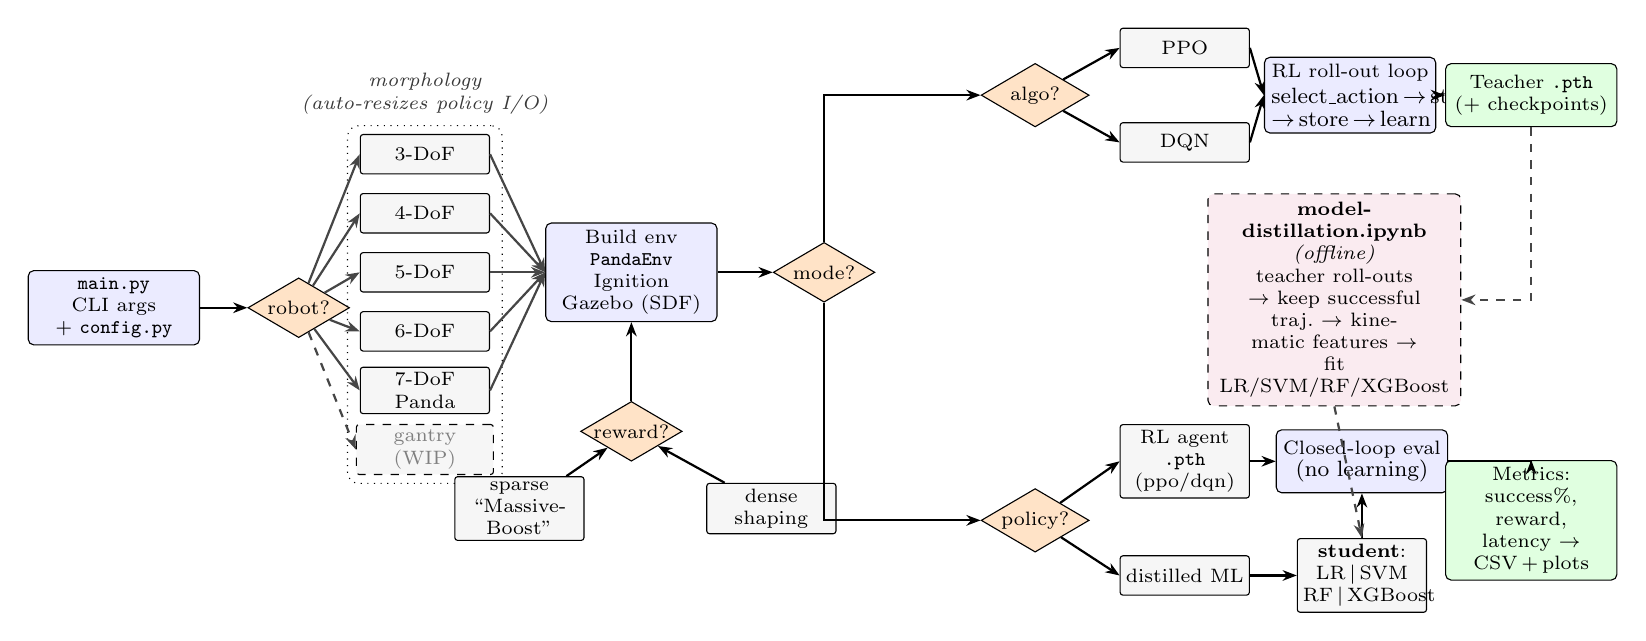
\begin{tikzpicture}[
  font=\scriptsize,
  >={Stealth[length=1.8mm]},
  stage/.style={rounded corners=2pt,draw,fill=blue!8,align=center,
                minimum height=8mm,inner sep=2.5pt,text width=20mm},
  dec/.style={draw,diamond,aspect=1.7,fill=orange!22,align=center,
              inner sep=0pt,minimum size=3mm,text width=10mm},
  alt/.style={draw,fill=gray!7,align=center,rounded corners=1pt,
              minimum height=5mm,inner sep=2pt,text width=15mm},
  store/.style={draw,fill=green!12,align=center,rounded corners=2pt,
                minimum height=8mm,inner sep=2.5pt,text width=20mm},
  distill/.style={draw,dashed,fill=purple!8,align=center,rounded corners=2pt,
                  inner sep=3pt,text width=30mm},
  flow/.style={->,thick},
  faint/.style={->,thick,gray!55!black,dashed},
  note/.style={font=\scriptsize\itshape,text=gray!45!black,align=center},
]
% ---------- shared entry spine ----------
\node[stage] (entry) at (0,0) {\textbf{\texttt{main.py}}\\CLI args\\$+$ \texttt{config.py}};
% robot decision + morphology stack
\node[dec,right=6mm of entry] (rdec) {robot?};
\node[alt] (r3) at (3.95,1.95) {3-DoF};
\node[alt] (r4) at (3.95,1.20) {4-DoF};
\node[alt] (r5) at (3.95,0.45) {5-DoF};
\node[alt] (r6) at (3.95,-0.30) {6-DoF};
\node[alt] (rp) at (3.95,-1.05) {7-DoF Panda};
\node[alt,dashed,text=gray,text width=16mm] (rt) at (3.95,-1.80) {gantry (WIP)};
\node[draw,dotted,rounded corners,fit=(r3)(r4)(r5)(r6)(rp)(rt),inner sep=3pt] (rbox) {};
\node[note,above=0.5pt of rbox] {morphology\\(auto-resizes policy I/O)};
% environment build
\node[stage,right=7mm of r5] (env) {Build env\\\texttt{PandaEnv}\\Ignition Gazebo (SDF)};
% reward decision feeding the env
\node[dec,below=10mm of env] (rwdec) {reward?};
\node[alt] (rw1) at (5.15,-2.55) {sparse\\``Massive-Boost''};
\node[alt] (rw2) at (8.35,-2.55) {dense\\shaping};
% mode decision
\node[dec,right=7mm of env] (mdec) {mode?};
% ---------- TRAIN lane (upper) ----------
\node[dec] (adec) at (11.7,2.7) {algo?};
\node[alt] (ppo) at (13.6,3.3) {PPO};
\node[alt] (dqn) at (13.6,2.1) {DQN};
\node[stage] (trloop) at (15.7,2.7)
   {RL roll-out loop\\\footnotesize select\_action\,$\to$\,step\\$\to$\,store\,$\to$\,learn};
\node[store] (teacher) at (18.0,2.7) {Teacher \texttt{.pth}\\(+ checkpoints)};
% ---------- TEST lane (lower) ----------
\node[dec] (pdec) at (11.7,-2.7) {policy?};
\node[alt] (rlag) at (13.6,-1.95) {RL agent\\\texttt{.pth} (ppo/dqn)};
\node[alt] (mlag) at (13.6,-3.4) {distilled ML};
\node[alt] (students) at (15.85,-3.4)
   {\textbf{student}: LR\,$|$\,SVM\\RF\,$|$\,XGBoost};
\node[stage] (evloop) at (15.85,-1.95) {Closed-loop eval\\\footnotesize(no learning)};
\node[store] (metrics) at (18.0,-2.7) {Metrics:\\success\%, reward,\\latency $\to$ CSV\,$+$\,plots};
% ---------- offline distillation bridge ----------
\node[distill] (distill) at (15.5,0.1)
   {\textbf{model-distillation.ipynb} \emph{(offline)}\\
    teacher roll-outs $\to$ keep successful\\
    traj.\ $\to$ kinematic features $\to$\\
    fit LR/SVM/RF/XGBoost};
% =================== edges ===================
\draw[flow] (entry) -- (rdec);
\foreach \n in {r3,r4,r5,r6,rp}{\draw[flow,gray!55!black] (rdec) -- (\n.west);}
\draw[faint] (rdec) -- (rt.west);
\foreach \n in {r3,r4,r5,r6,rp}{\draw[flow,gray!55!black] (\n.east) -- (env.west);}
\draw[flow] (rw1) -- (rwdec);
\draw[flow] (rw2) -- (rwdec);
\draw[flow] (rwdec) -- (env);
\draw[flow] (env) -- (mdec);
% mode -> lanes
\draw[flow] (mdec.north) |- (adec.west);
\draw[flow] (mdec.south) |- (pdec.west);
% train lane
\draw[flow] (adec) -- (ppo.west);
\draw[flow] (adec) -- (dqn.west);
\draw[flow] (ppo.east) -- (trloop.west);
\draw[flow] (dqn.east) -- (trloop.west);
\draw[flow] (trloop) -- (teacher);
% test lane: both RL agent and distilled student feed the same eval loop
\draw[flow] (pdec) -- (rlag.west);
\draw[flow] (pdec) -- (mlag.west);
\draw[flow] (rlag.east) -- (evloop.west);
\draw[flow] (mlag) -- (students);
\draw[flow] (students.north) -- (evloop.south);
\draw[flow] (evloop) -| (metrics.north);
% distillation bridge: teacher -> notebook -> students
\draw[faint] (teacher.south) |- (distill.east);
\draw[faint] (distill.south) -- (students.north);
\end{tikzpicture}}
\caption{Configuration-driven control flow of the framework, read left to right.
A single \texttt{main.py}/\texttt{config.py} entry point branches (orange
decisions) on \emph{morphology} (3--7~DoF, auto-resizing the policy I/O), on the
\emph{reward}, and on the \emph{mode}. \textbf{Train} selects a learning
algorithm (PPO/DQN) and produces a teacher checkpoint; an offline notebook
distils that teacher into compact LR/SVM/RF/XGBoost students. \textbf{Test}
runs either the RL teacher or any distilled student through the same
closed-loop evaluator. Each stacked group is a set of mutually exclusive
(if/else) routes.}
\label{fig:framework}
\end{figure*}

\subsection{State and action formulation}
The state $s_t\in\mathbb{R}^{n+3}$ concatenates the $n$ joint angles, normalized
to $[-1,1]$ by their physical limits, with the 3-D target position. The policy
emits a normalized action $a_t\in[-1,1]^n$ that is denormalized to absolute joint
targets,
\begin{equation}
a_{\text{real}} = l_{\text{low}} + \tfrac{(a_{\text{norm}}+1)}{2}\,(l_{\text{high}}-l_{\text{low}}),
\label{eq:denorm}
\end{equation}
so $-1\!\mapsto\!l_{\text{low}}$ and $+1\!\mapsto\!l_{\text{high}}$ regardless of
morphology.

\subsection{Sparse ``Massive-Boost'' reward}
The contact-rich task is to push an object off a table edge. A high-magnitude
sparse reward---$+100$ on first displacing the object and $+1000$ on success---is
used; dense distance shaping was found to induce a hovering local optimum. This
reward defines which episodes count as ``successful'' and are retained for
distillation.

\subsection{PPO teacher}
The teacher is a standard Proximal Policy Optimization agent \cite{schulman} with
a Gaussian actor and a separate critic, each a two-layer ($128{\times}128$)
$\tanh$ multilayer perceptron; the $\tanh$ output naturally respects the $[-1,1]$
action range. The same algorithm and hyperparameters are used for all
morphologies. Teacher training curves are shown in Fig.~\ref{fig:teacher}.

\begin{figure}[t]
\centering
\begin{subfigure}[b]{0.49\columnwidth}
  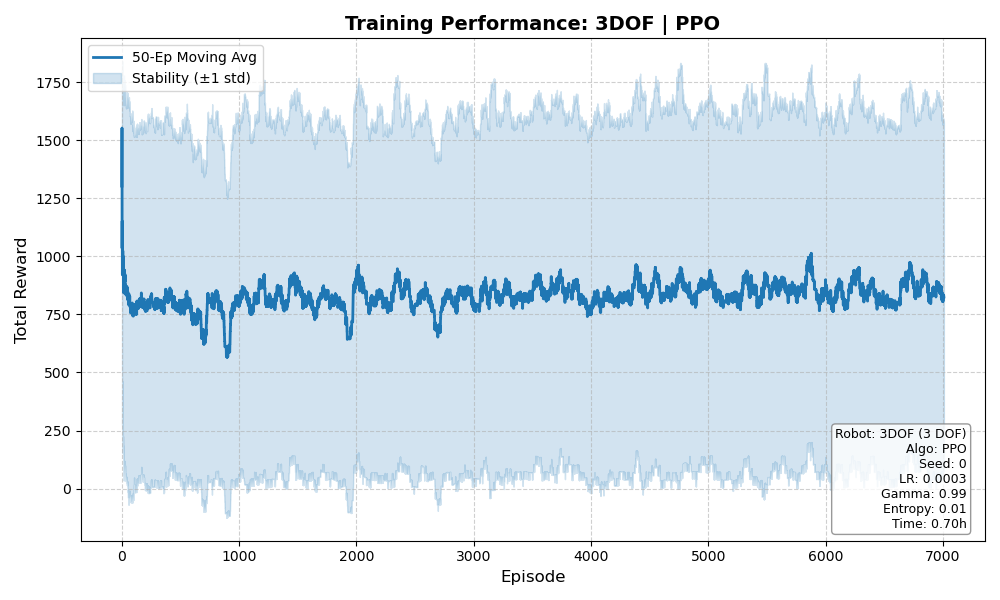
\includegraphics[width=\textwidth]{plot_3dof_ppo_sparse_s0_22-03-2026_20-25.png}
  \caption{3-DoF}
\end{subfigure}\hfill
\begin{subfigure}[b]{0.49\columnwidth}
  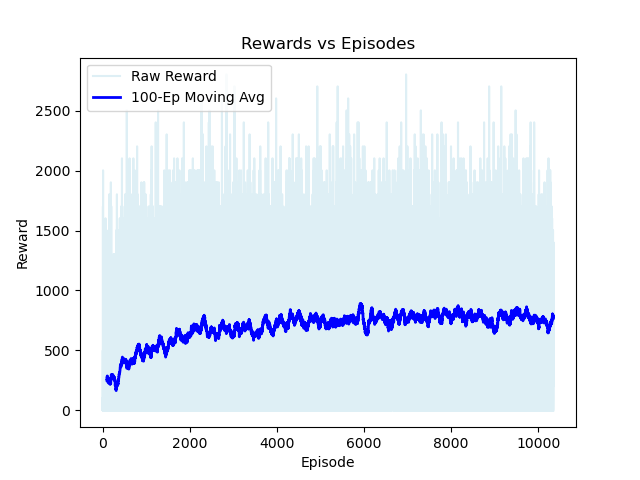
\includegraphics[width=\textwidth]{plot_panda_ppo_sparse_s42_17-03-2026_23-15.png}
  \caption{7-DoF Panda}
\end{subfigure}
\caption{Representative sparse-PPO teacher training curves (moving-average reward,
shaded $\pm1$ std). Lower-DoF arms converge faster.}
\label{fig:teacher}
\end{figure}

%==============================================================================
\section{Policy Distillation Methodology}
%==============================================================================
Fig.~\ref{fig:pipeline} summarizes the pipeline: roll out the frozen teacher,
filter successful trajectories, engineer kinematic features, fit per-morphology
students to delta-action targets, and redeploy the students in closed loop.

\begin{figure*}[t]
\centering
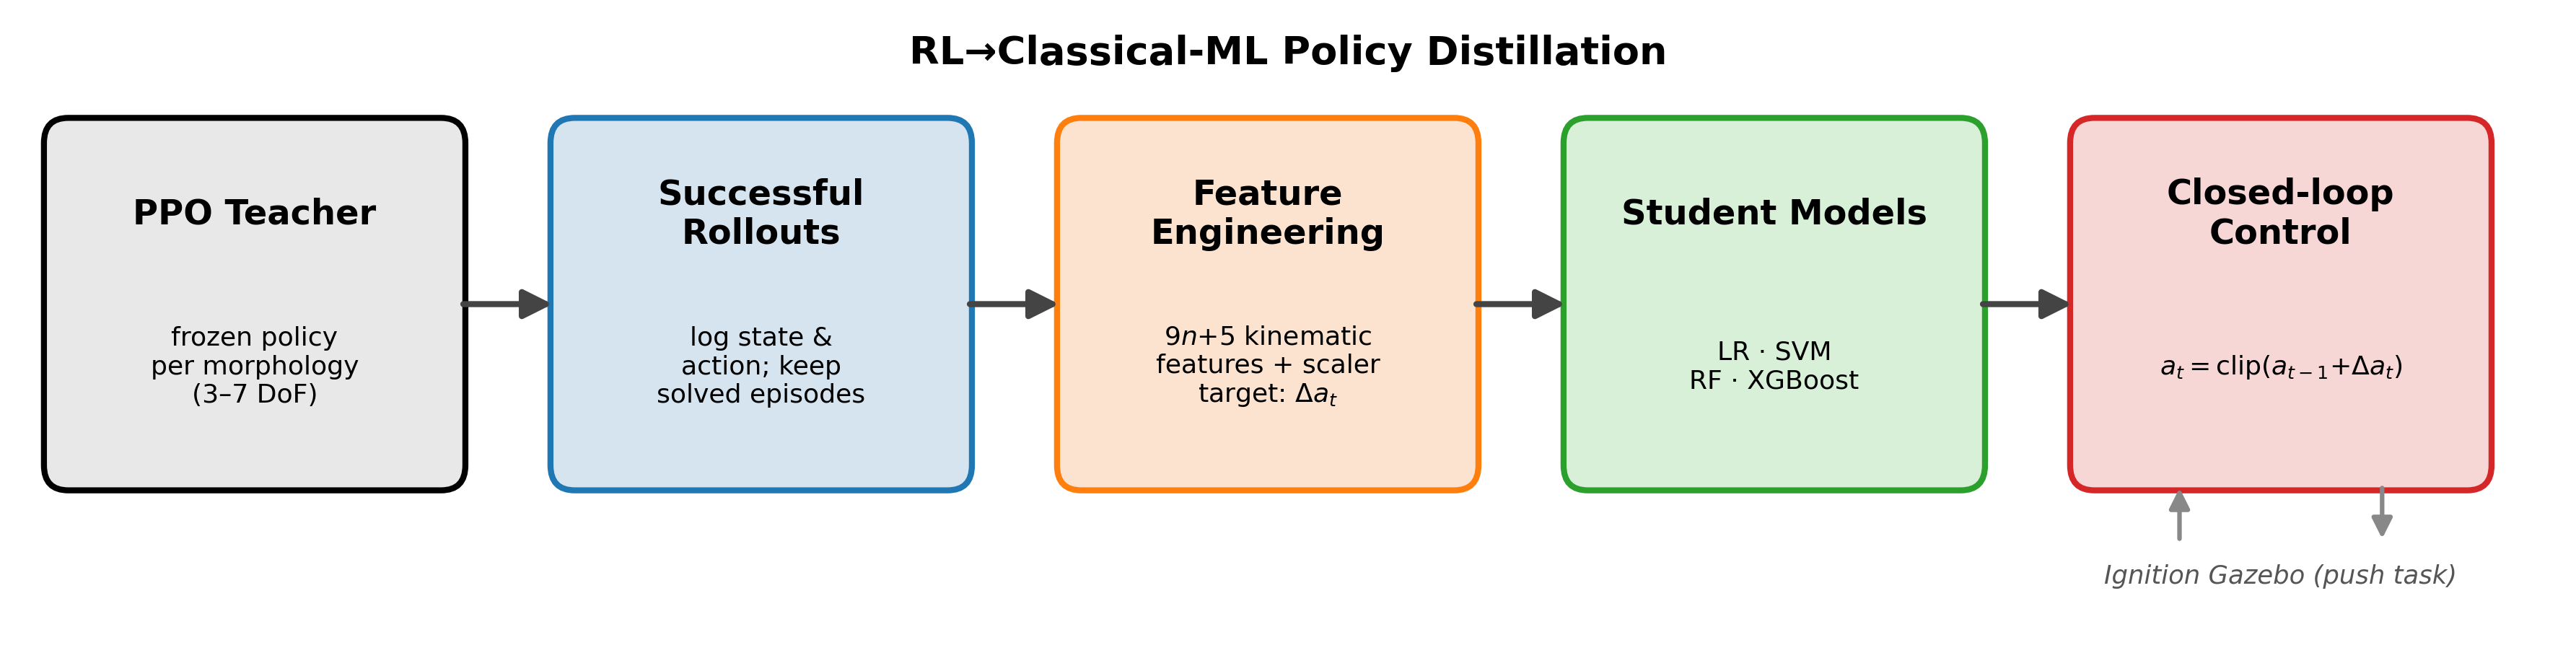
\includegraphics[width=0.92\textwidth]{distillation_pipeline.png}
\caption{Distillation pipeline: a frozen PPO teacher generates trajectories that
supervise compact student models, which are then deployed as standalone
closed-loop controllers.}
\label{fig:pipeline}
\end{figure*}

\subsection{Dataset generation}
For each morphology the trained teacher is evaluated for many episodes and every
step is logged: episode and step indices, the (denormalized) joint angles, the
target position, and the executed normalized action. Only steps belonging to
\emph{successful} episodes are retained, so the students imitate competent
behavior rather than exploratory failure.

\subsection{Kinematic feature engineering}
Each retained step is expanded into a feature vector of dimension $9n+5$, where
$n$ is the DoF. Five \emph{task} features capture the goal geometry,
\begin{equation}
\mathbf{e}=\mathbf{p}_{\text{obj}}-\mathbf{p}^{*},\quad
d=\lVert\mathbf{e}\rVert,\quad
\rho=\tfrac{\text{step}}{\text{episode length}},
\end{equation}
i.e. the per-axis error $\mathbf{e}=(e_x,e_y,e_z)$ to a fixed reference
$\mathbf{p}^{*}=(0.5,0,0.5)$, its norm $d$, and a normalized progress $\rho$.
For each joint $i$ we add nine \emph{kinematic} features: the angle encodings
$\sin\theta_i,\cos\theta_i$; finite-difference velocity, acceleration and jerk
\begin{equation}
v_i=\tfrac{\Delta\theta_i}{\Delta t},\;
\alpha_i=\tfrac{\Delta v_i}{\Delta t},\;
j_i=\tfrac{\Delta \alpha_i}{\Delta t};
\end{equation}
the cross term $v_i\alpha_i$; two action lags $a_i^{t-1},a_i^{t-2}$; and the
velocity lag $v_i^{t-1}$. All features are standardized by a
\texttt{StandardScaler} fit on the training split and stored alongside each model.

\subsection{Delta-action target}
Rather than regressing the absolute command, each student predicts the
\emph{change} in the normalized action,
\begin{equation}
y_i^{t}=\Delta a_i^{t}=a_i^{t}-a_i^{t-1},
\label{eq:delta}
\end{equation}
which is smoother and better conditioned than the raw command. Four multi-output
regressors are trained per morphology: LR, an RBF-kernel SVM, an RF
($100$ trees), and XGBoost ($200$ trees, depth $6$, learning rate $0.1$); SVM,
RF, and XGBoost are wrapped per output dimension.

\subsection{Closed-loop deployment}
At deployment the student is queried every control step. From the live
observation we reconstruct the same features---denormalizing joints exactly as in
\eqref{eq:denorm}---predict $\Delta a^{t}$, and integrate
\begin{equation}
a^{t}=\mathrm{clip}\!\left(a^{t-1}+\Delta a^{t},\,-1,\,1\right),
\label{eq:integrate}
\end{equation}
maintaining the per-episode recurrence (joint/velocity/acceleration and the two
action lags), reset at every episode. The clip keeps the command---and hence the
lagged-action features---inside the training range.

\paragraph*{A note on the time step}
The velocity/acceleration/jerk features are time-derivatives whose $\Delta t$ was
derived from per-step wall-clock latency during data collection. That quantity is
both non-causal (it depends on the step being timed) and machine-dependent, so it
cannot be reproduced faithfully online. We therefore use a fixed
$\Delta t$ equal to the training floor, which keeps these features within the
range expected by the scaler and renders the controller deterministic and
reproducible.

%==============================================================================
\section{Experimental Setup}
%==============================================================================
The teacher and all students are evaluated in Ignition Gazebo on the pushing task
under the sparse reward. For each morphology and each model we run a fixed number
of evaluation episodes from identical seeds. Unless stated otherwise the PPO
teacher is run with its native stochastic policy (actions sampled from the
Gaussian, as during training); the distilled students are deterministic. On the
7-DoF arm we additionally report a \emph{greedy} teacher evaluation (mean action,
no sampling), which is the deployment-relevant mode and isolates how much of the
teacher's success is exploration-noise-borrowed. We report:
\begin{itemize}
  \item \textbf{Fidelity ($R^2$):} coefficient of determination of the predicted
        delta-action on a held-out split of the teacher rollouts.
  \item \textbf{Task success:} fraction of episodes in which the object is pushed
        off the table, plus the cumulative ``successes vs.\ step'' curve.
  \item \textbf{Footprint:} serialized model size.
  \item \textbf{Latency:} mean wall-clock time of a single-sample prediction
        (scaler transform $+$ model inference) on CPU.
\end{itemize}
All metrics are reported as measured: footprint and latency from the serialized
models, fidelity from the distillation test split, and task success from
closed-loop evaluation over $100$ episodes per cell at a fixed seed.

%==============================================================================
\section{Results and Discussion}
%==============================================================================

% Both wide comparison floats are declared early (in citation order) so they
% land beside their discussion in the closed-loop subsection rather than being
% pushed past the references onto the final page.
\begin{figure*}[t]
\centering
\begin{subfigure}[b]{0.32\textwidth}
  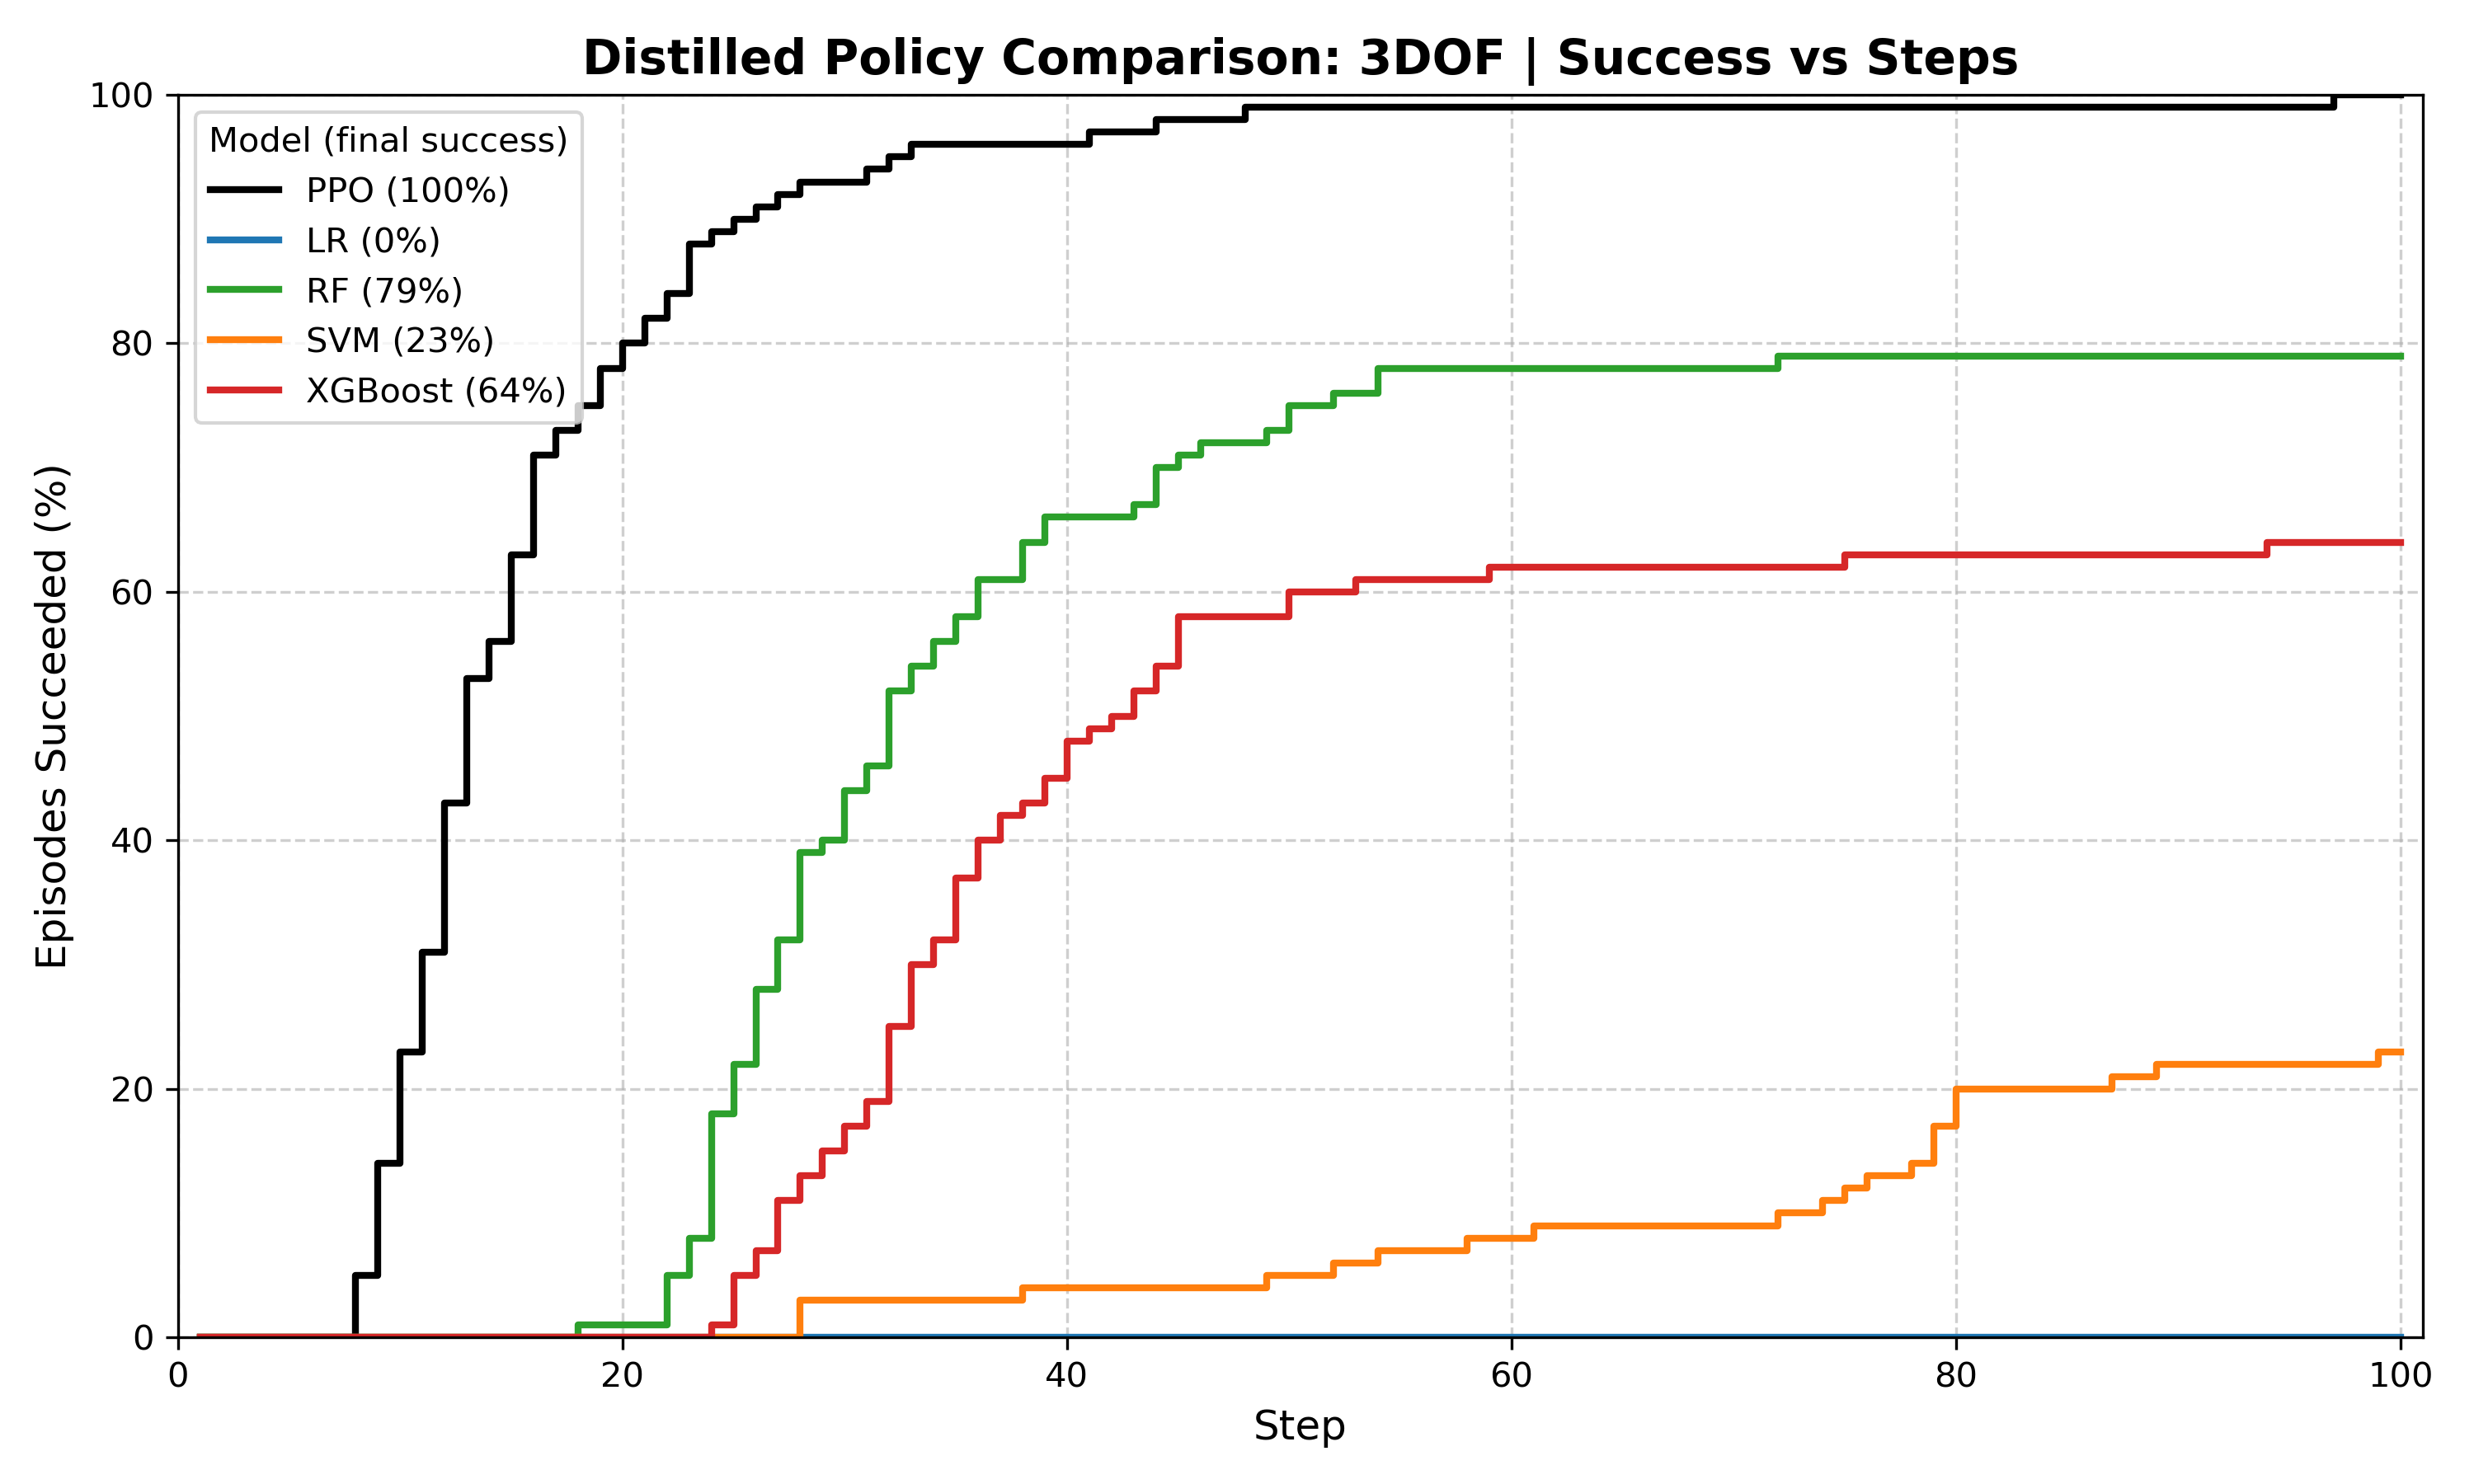
\includegraphics[width=\textwidth]{compare_3dof_cdf.png}\caption{3-DoF}
\end{subfigure}\hfill
\begin{subfigure}[b]{0.32\textwidth}
  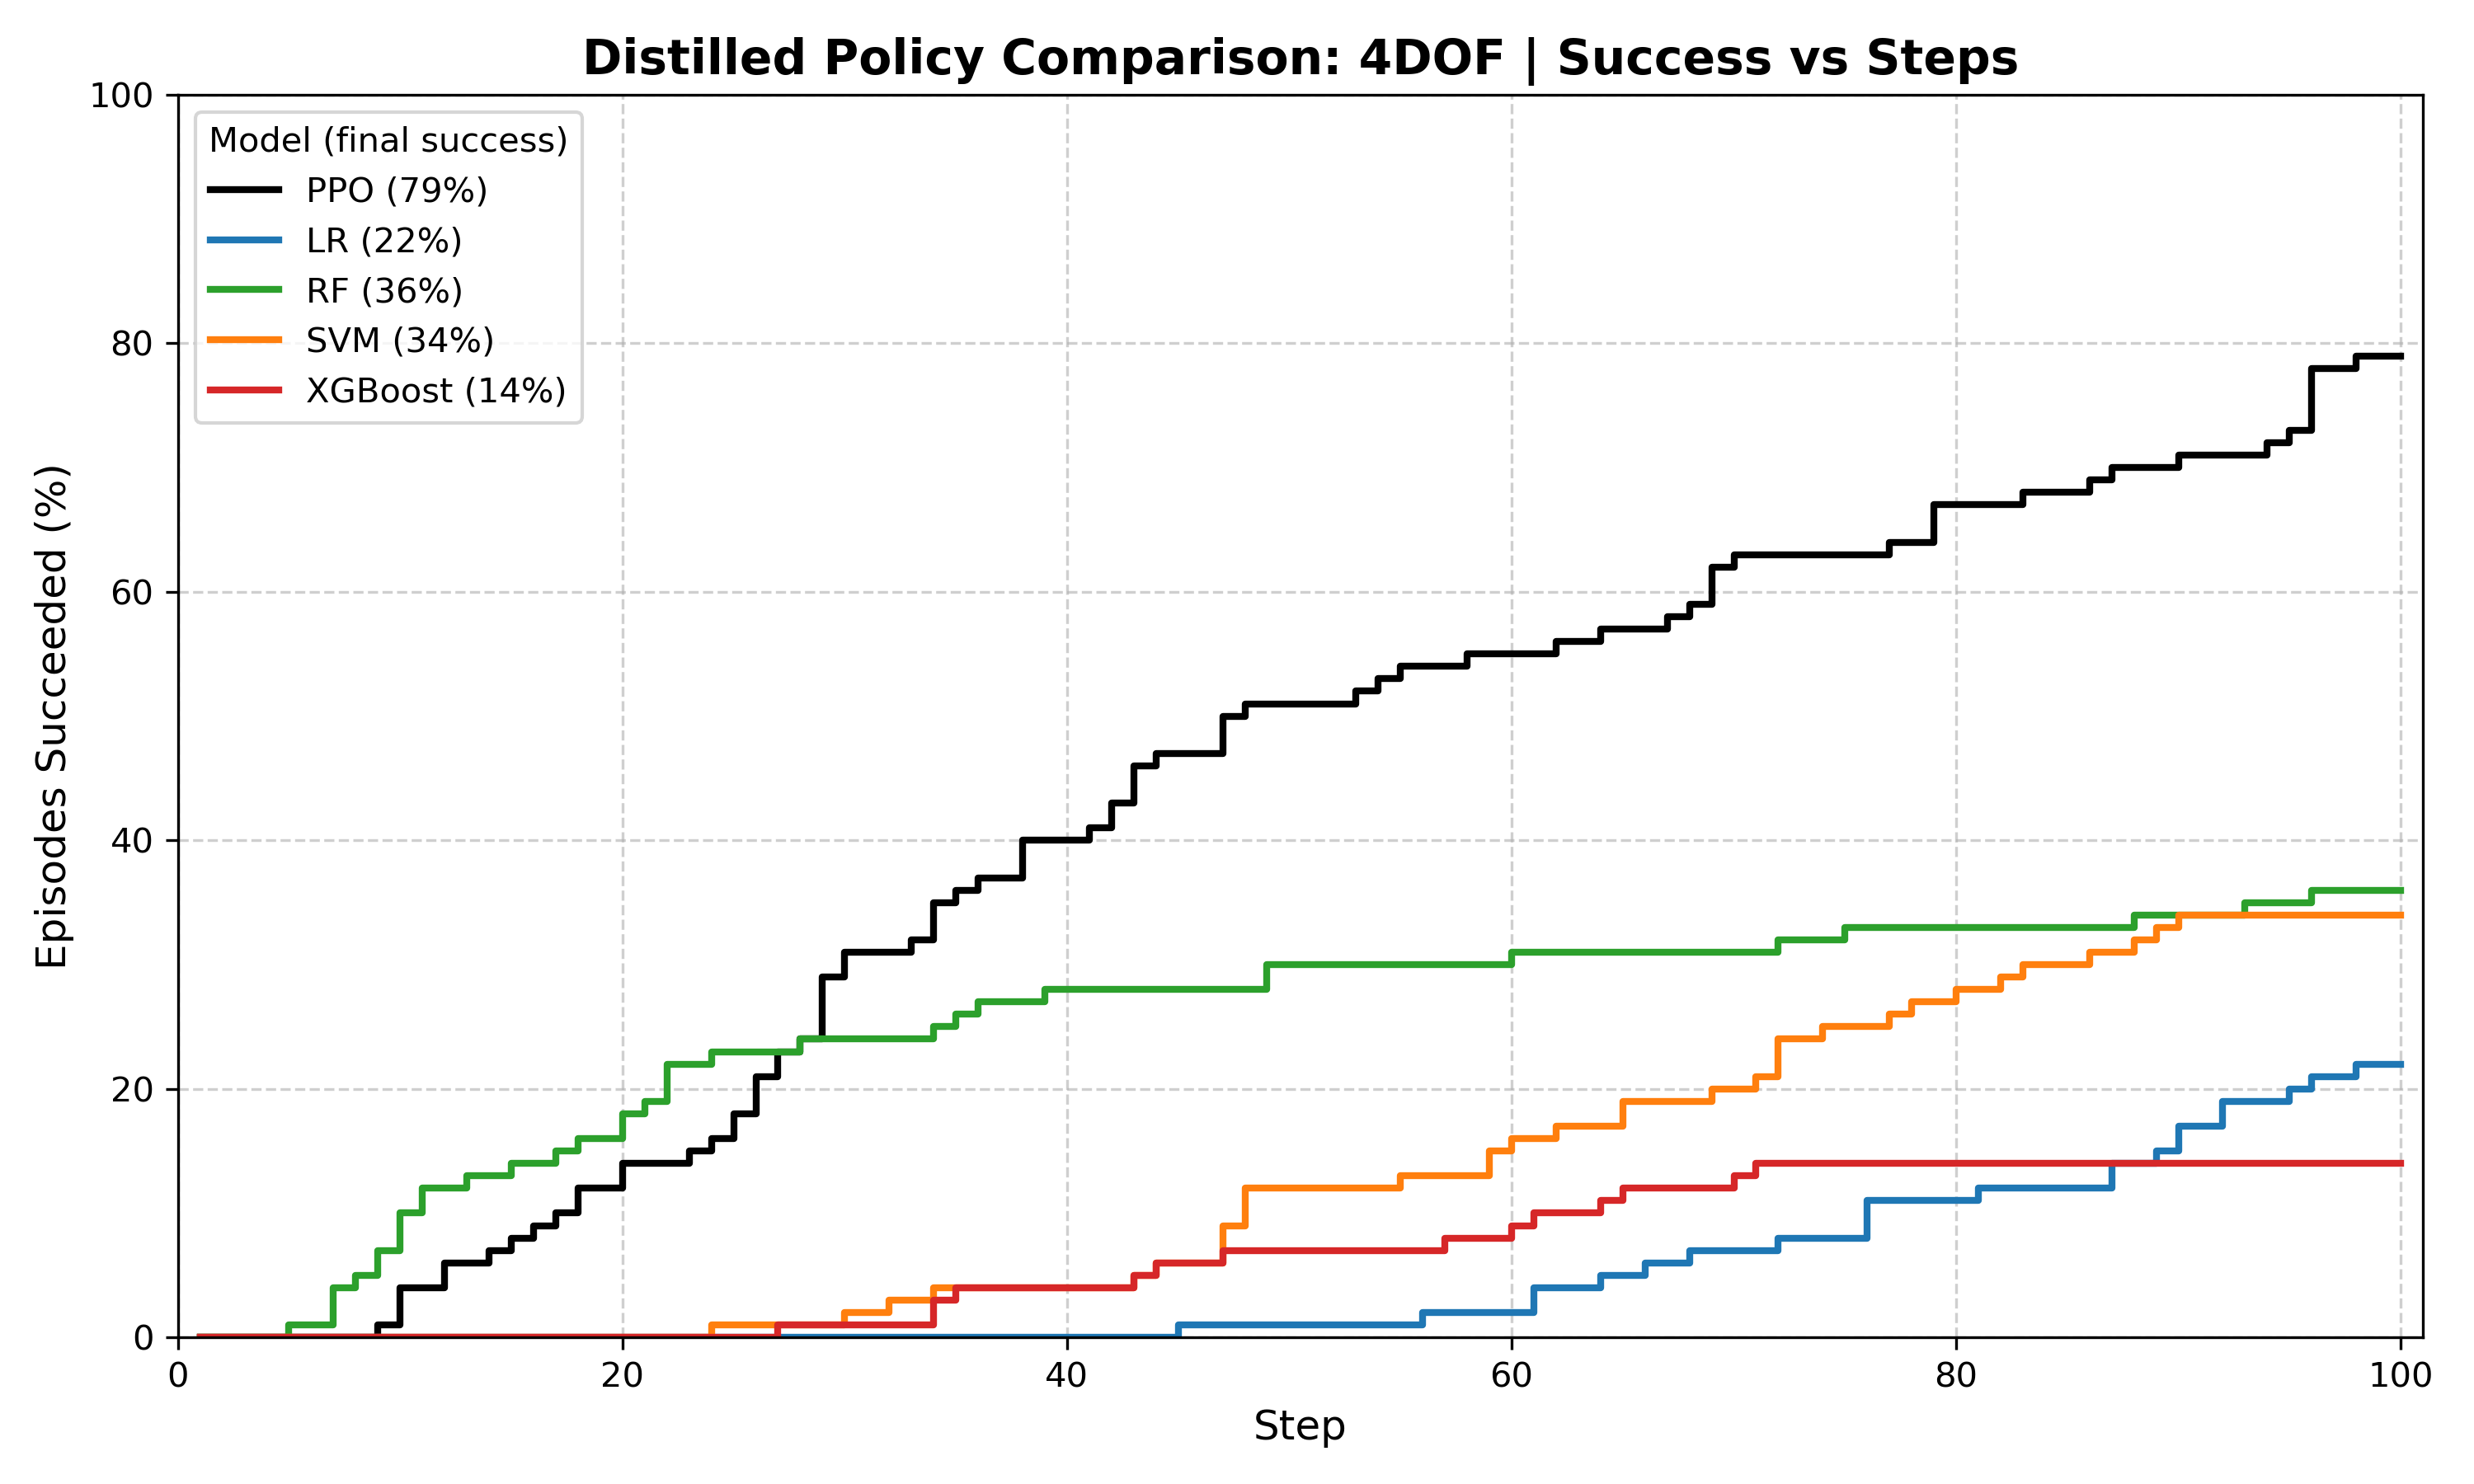
\includegraphics[width=\textwidth]{compare_4dof_cdf.png}\caption{4-DoF}
\end{subfigure}\hfill
\begin{subfigure}[b]{0.32\textwidth}
  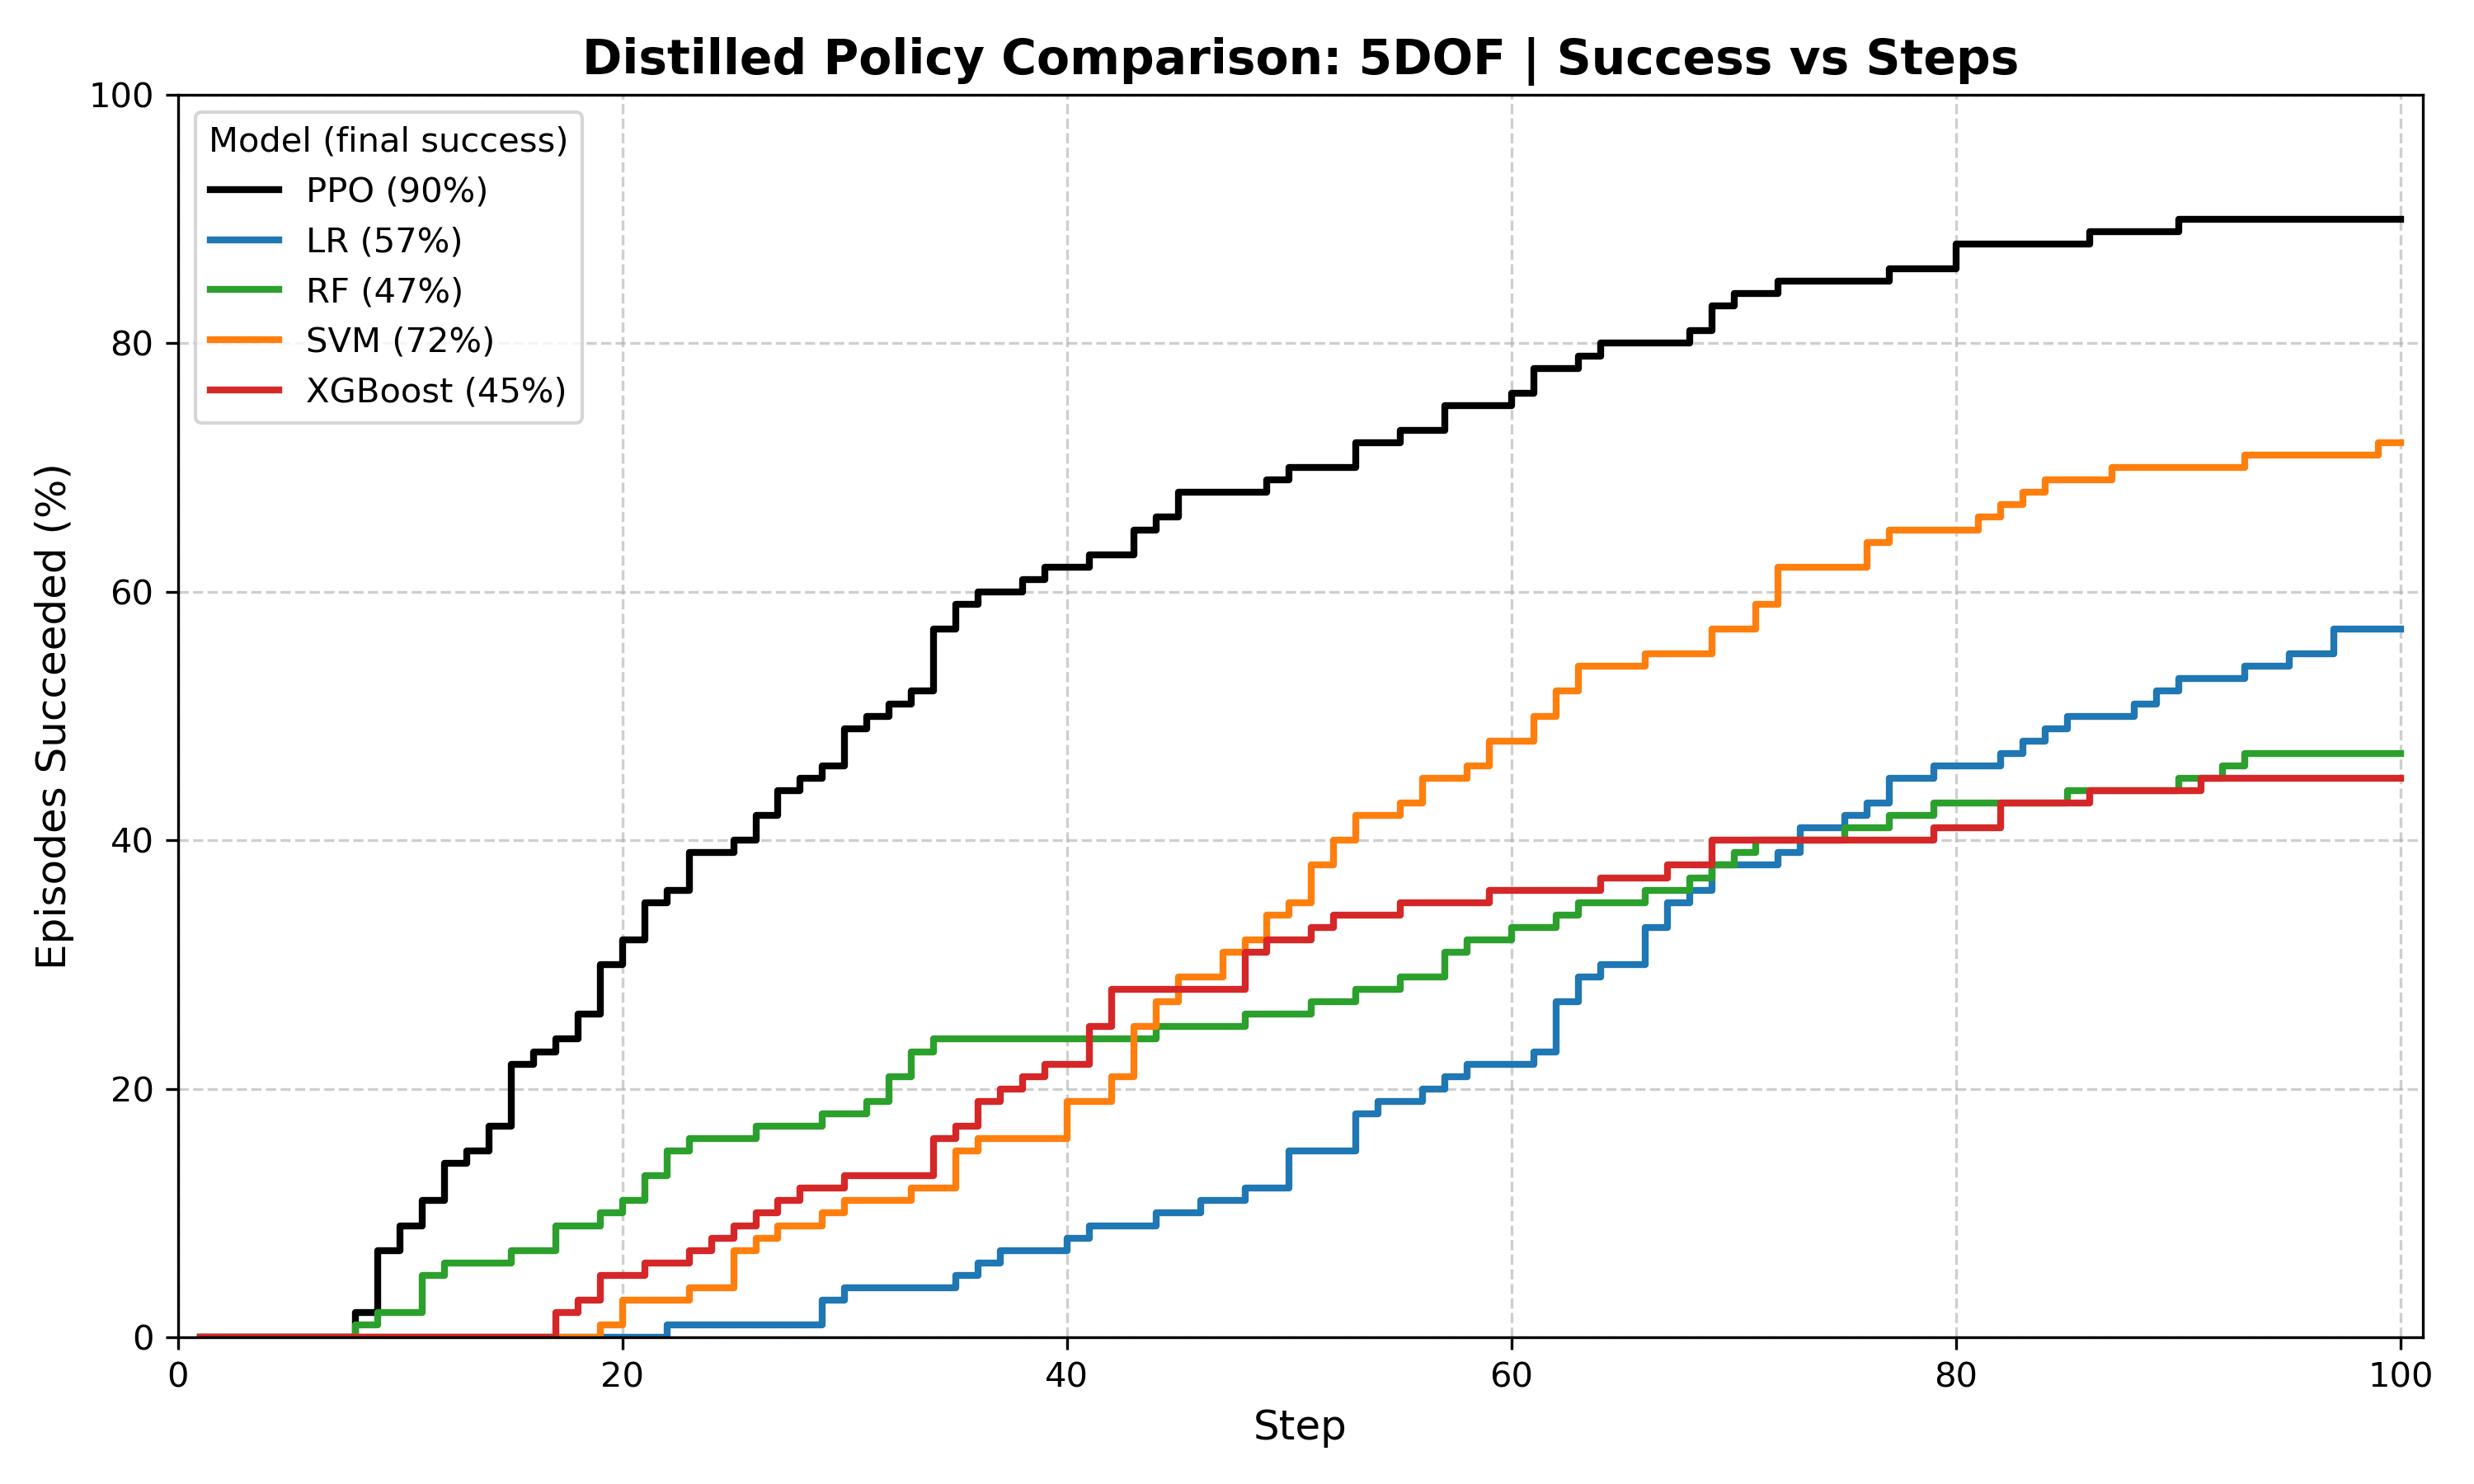
\includegraphics[width=\textwidth]{compare_5dof_cdf.png}\caption{5-DoF}
\end{subfigure}

\vspace{0.35cm}
\begin{subfigure}[b]{0.32\textwidth}
  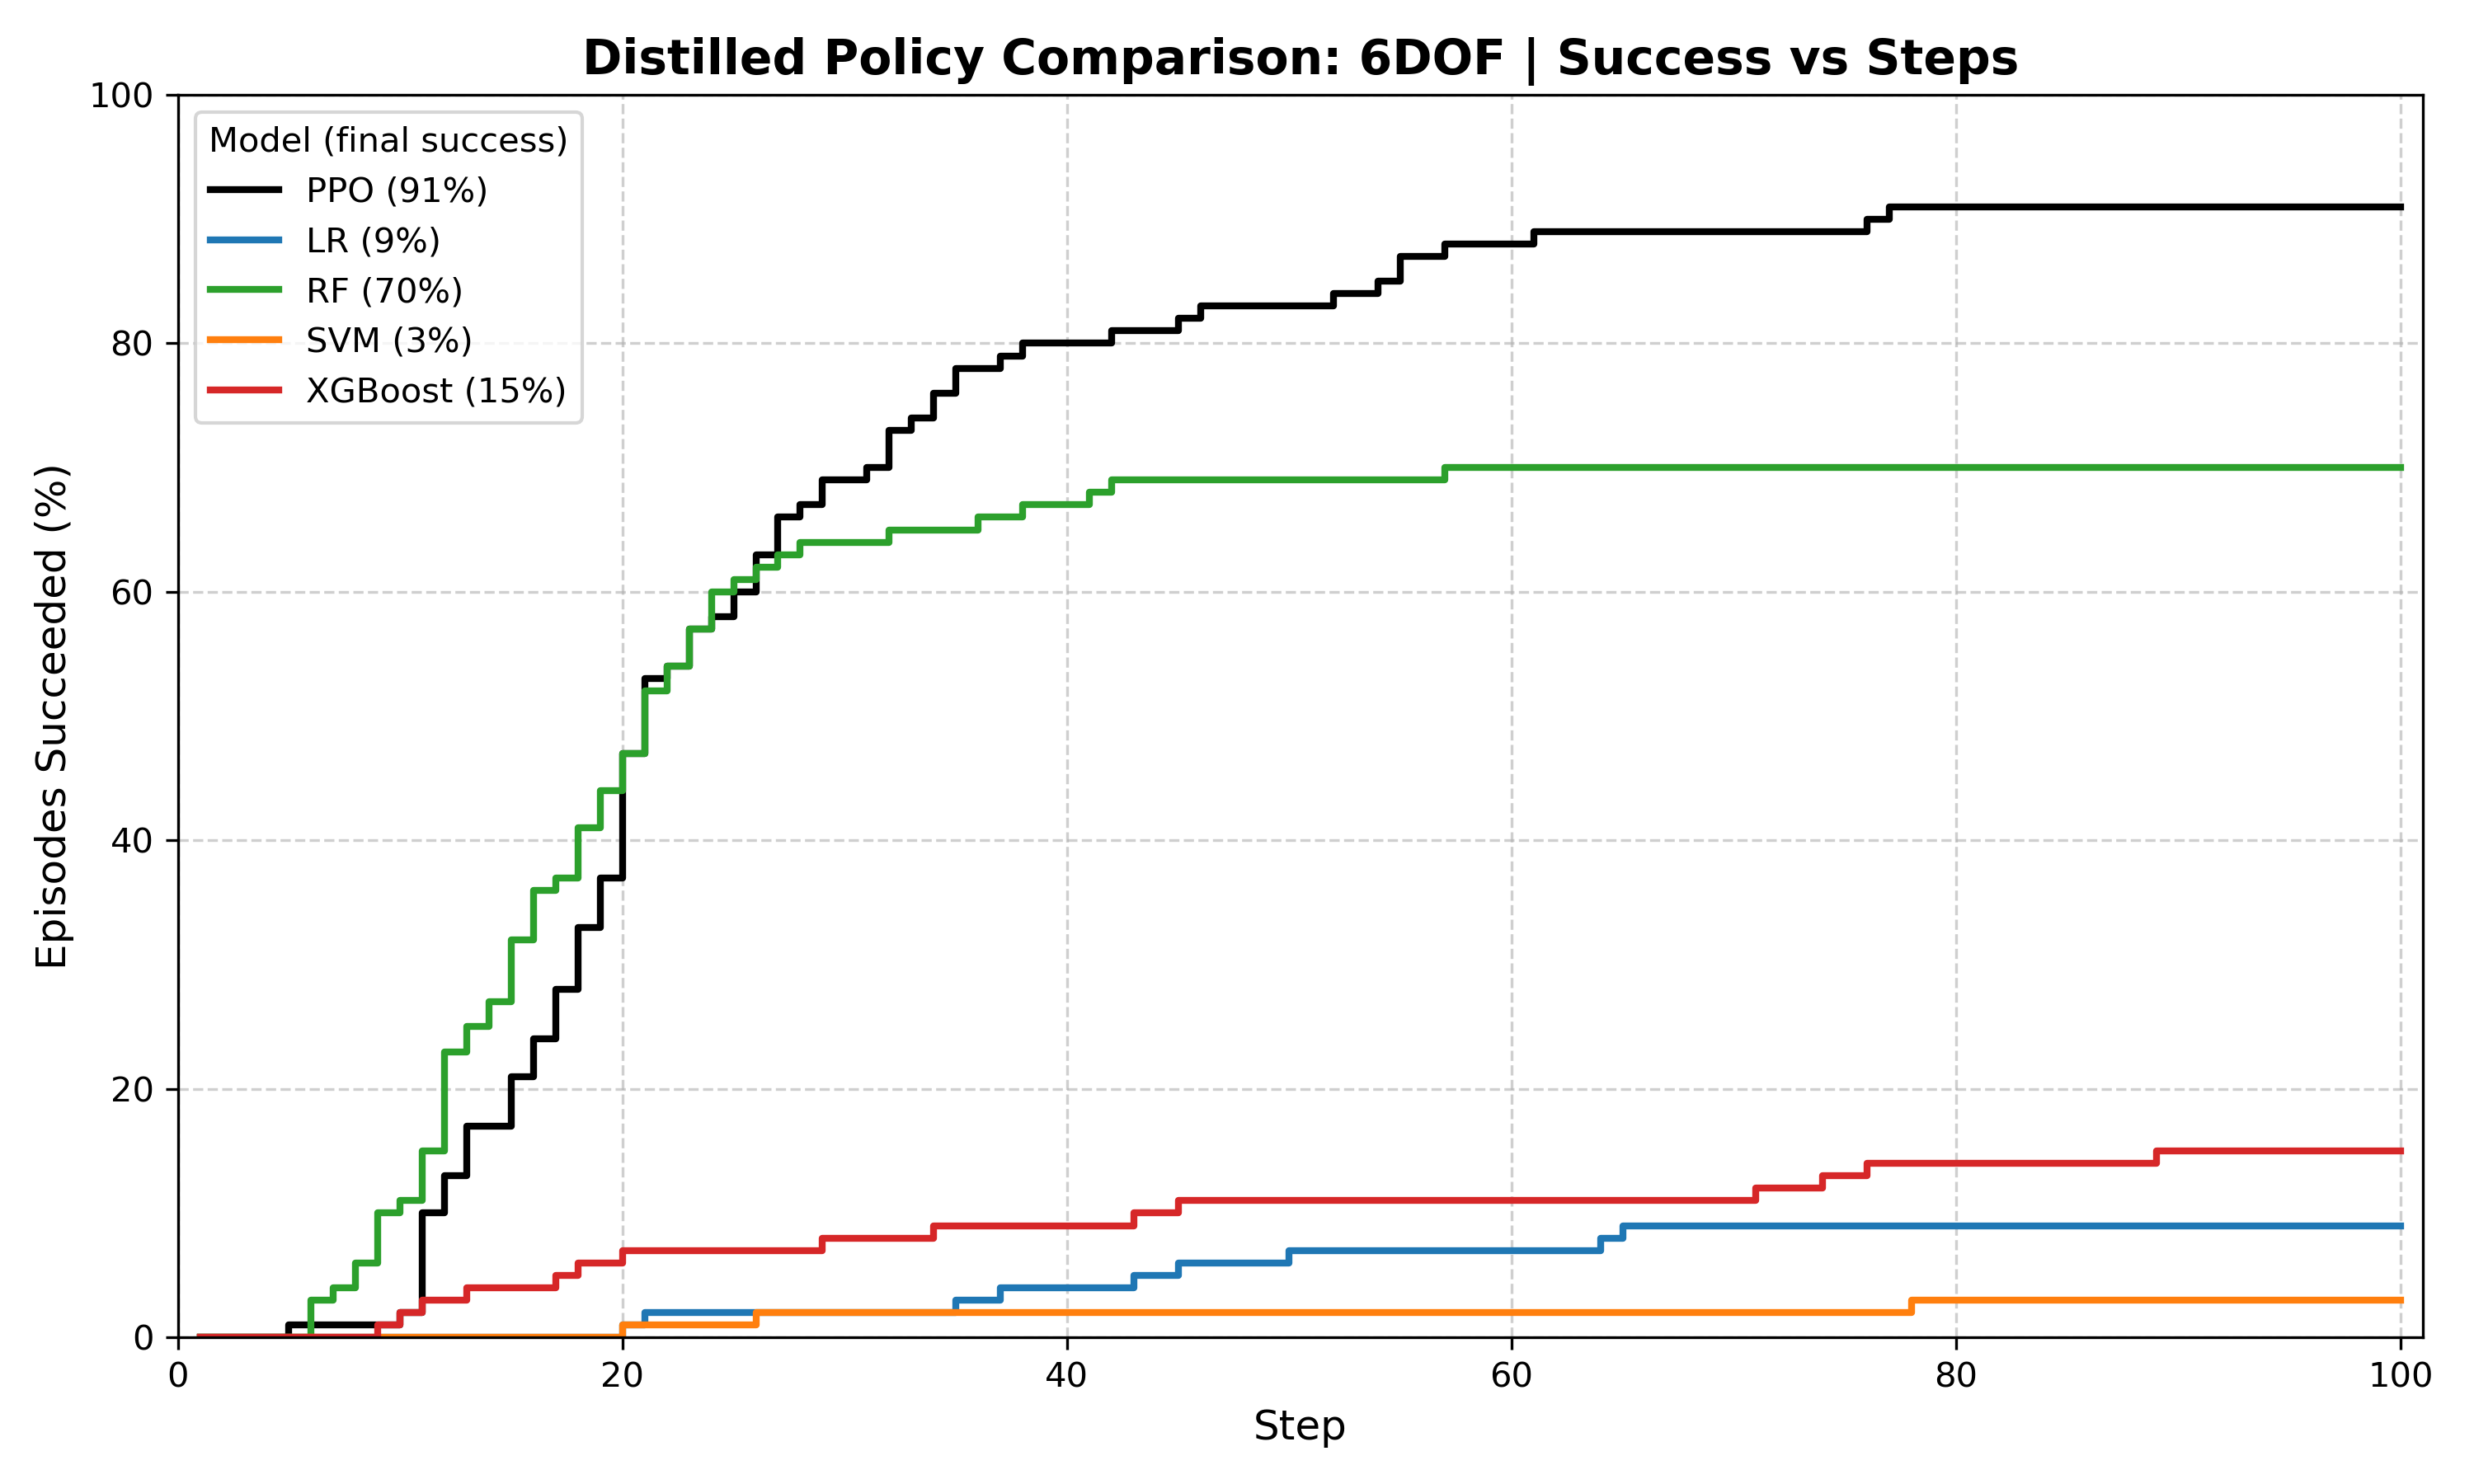
\includegraphics[width=\textwidth]{compare_6dof_cdf.png}\caption{6-DoF}
\end{subfigure}\hfill
\begin{subfigure}[b]{0.32\textwidth}
  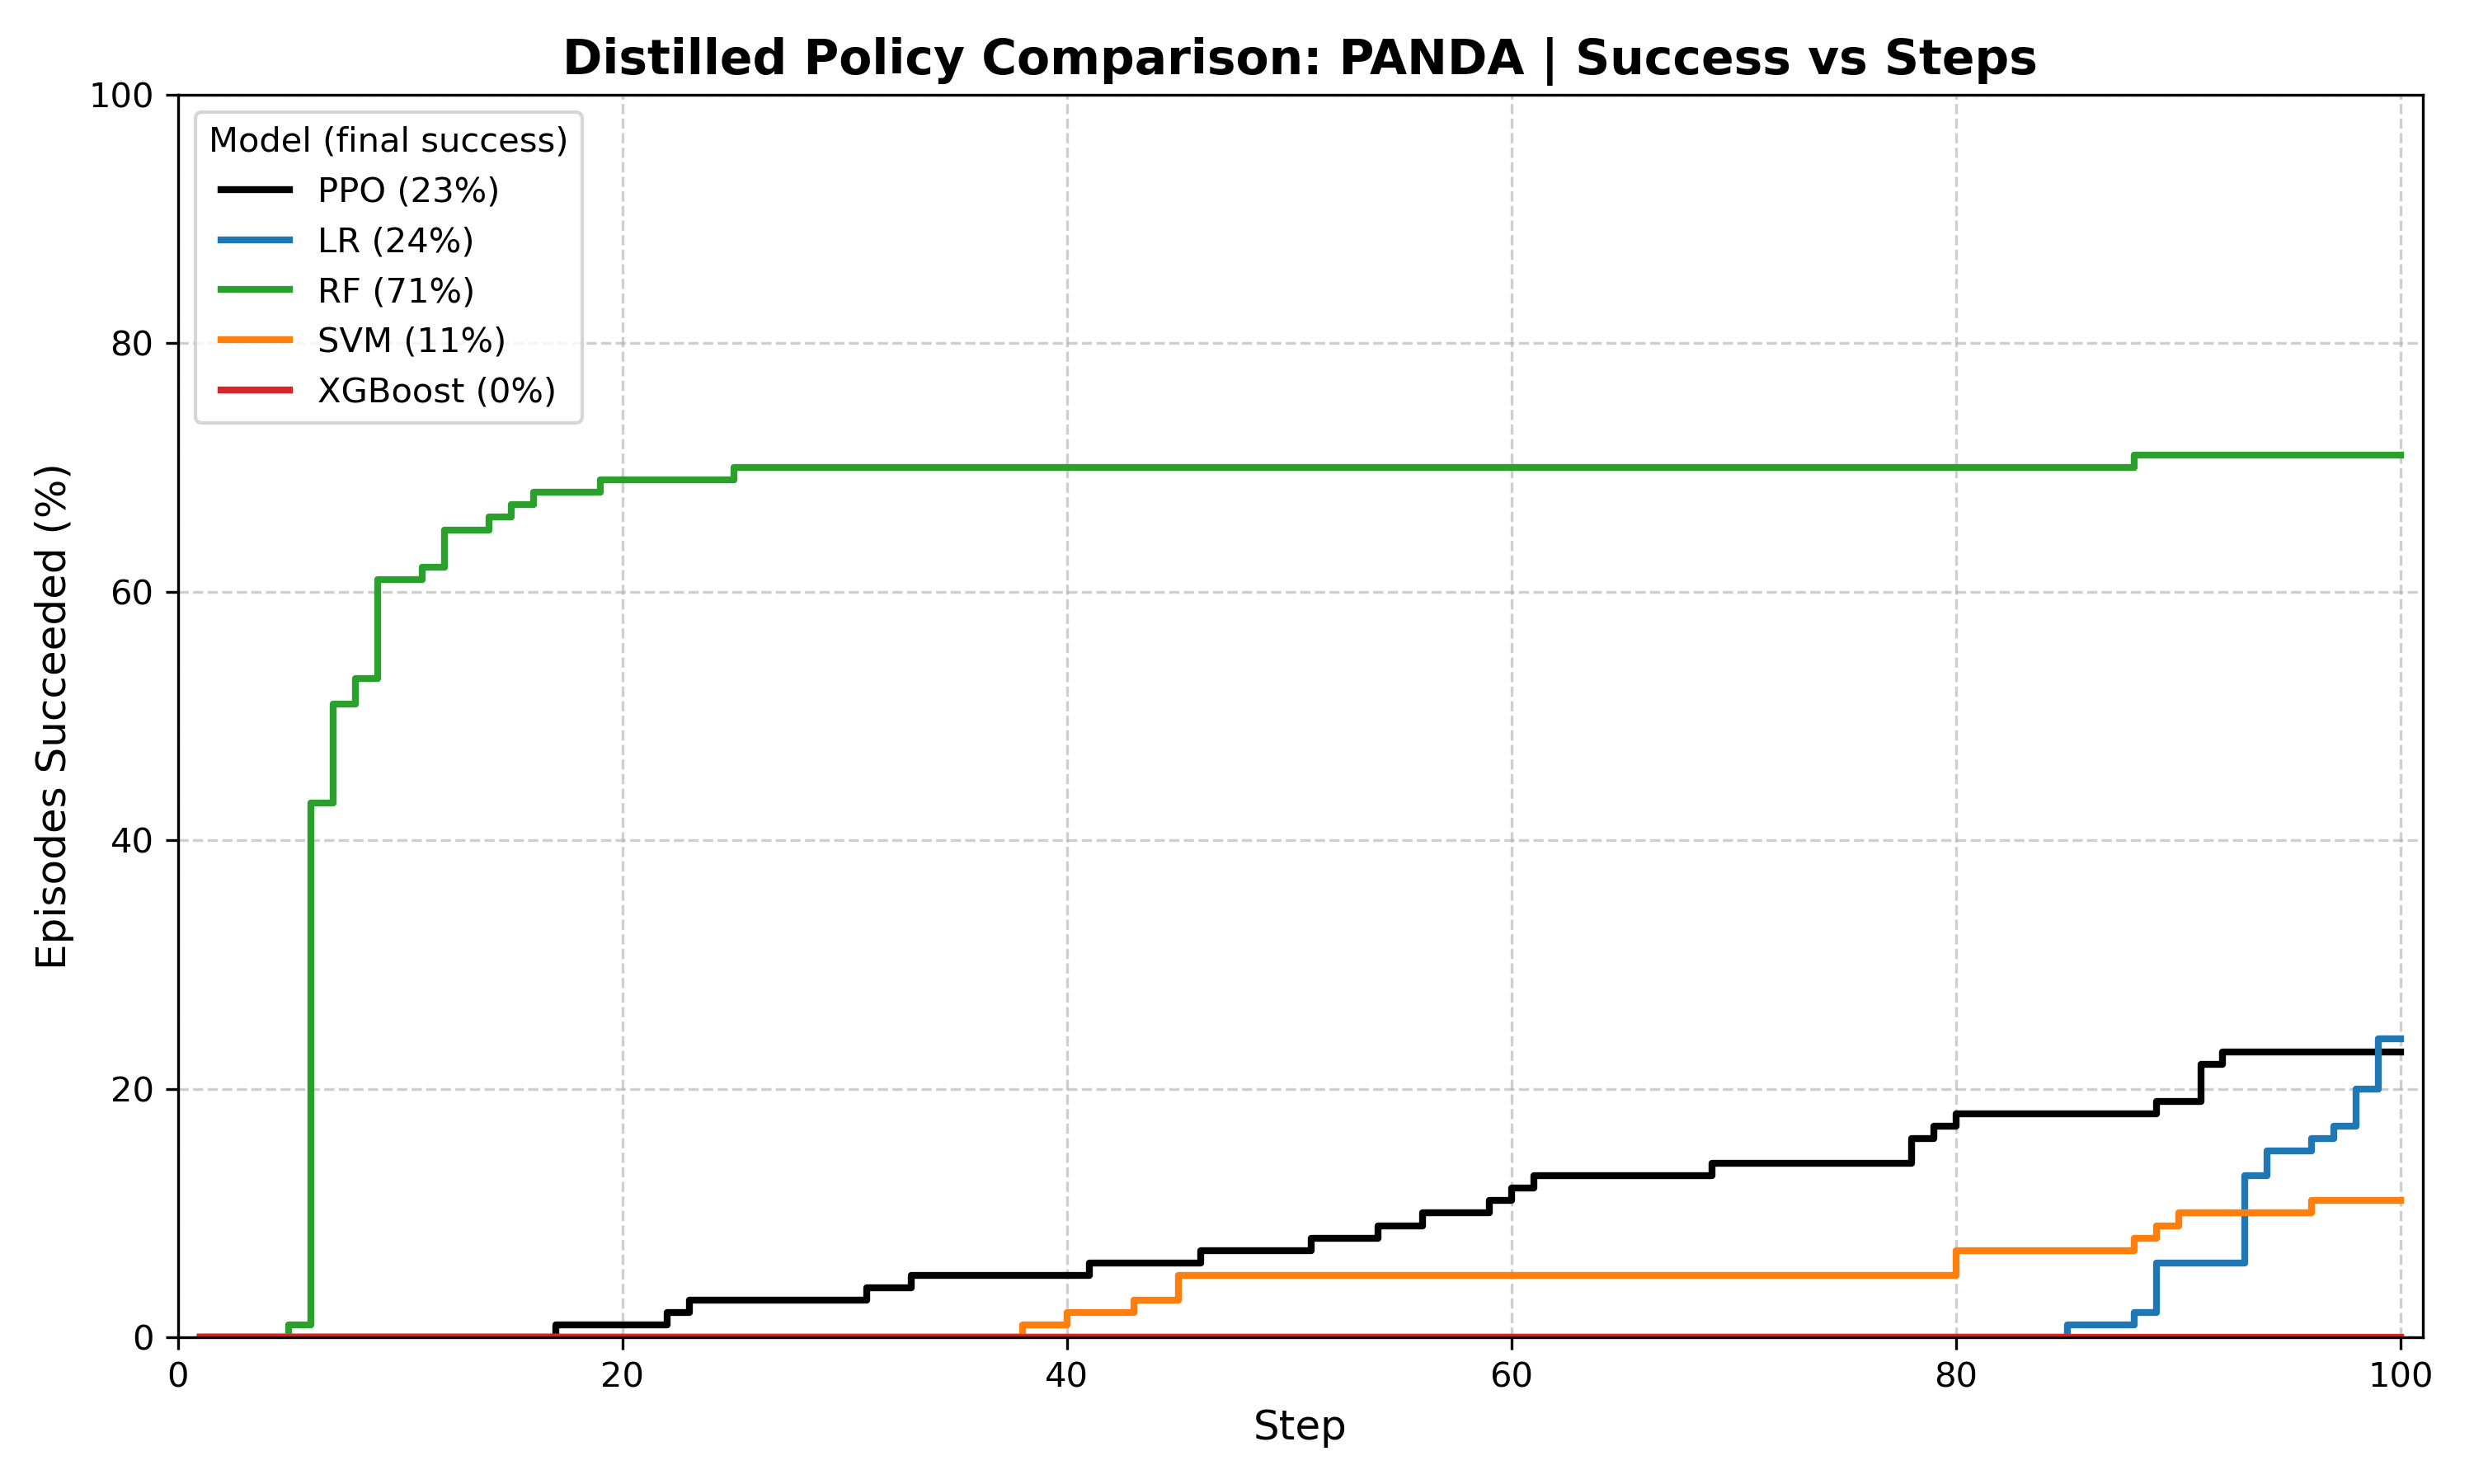
\includegraphics[width=\textwidth]{compare_panda_cdf.png}\caption{7-DoF (Panda)}
\end{subfigure}\hfill
\begin{subfigure}[b]{0.32\textwidth}
  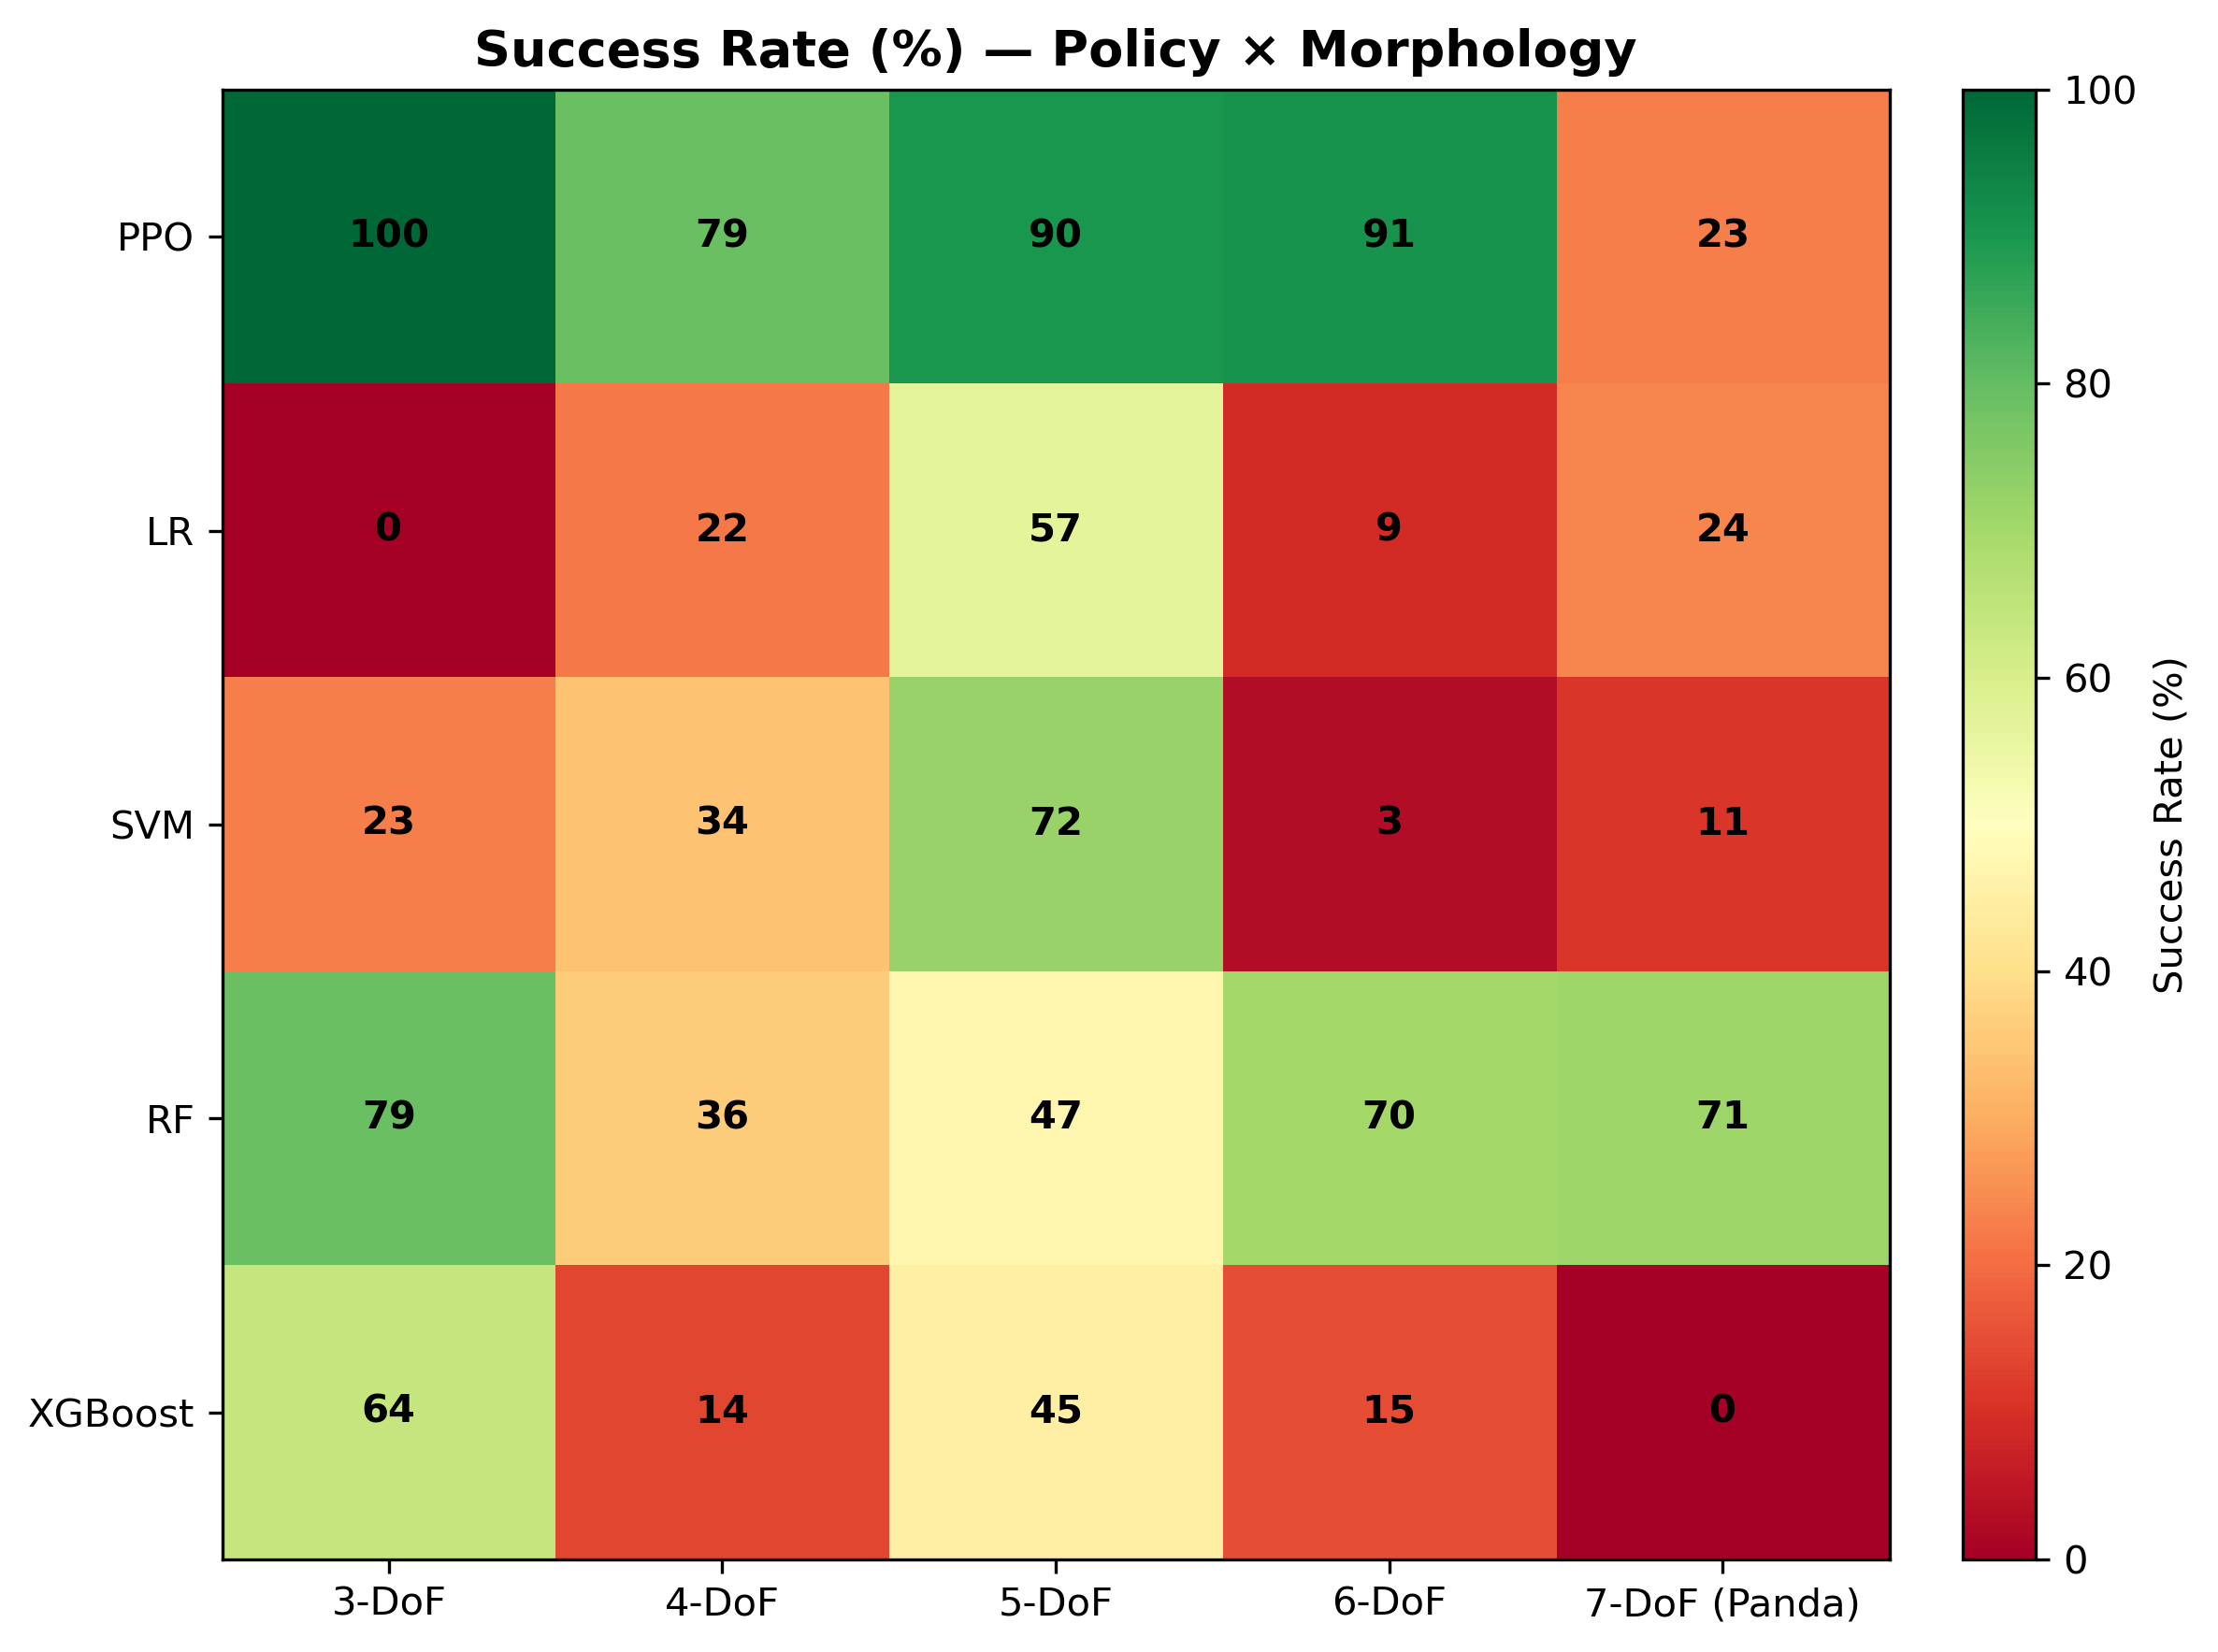
\includegraphics[width=\textwidth]{compare_all_success_heatmap.png}\caption{Success-rate matrix}
\end{subfigure}
\caption{Per-morphology closed-loop comparison. (a)--(e) Cumulative fraction of
episodes solved by a given step, one curve per policy (steeper/higher is better);
(f) the full success-rate matrix as a heatmap. The teacher leads on the low-DoF
arms, but on the 7-DoF Panda the random-forest student dominates.}
\label{fig:overlay}
\end{figure*}

\begin{figure*}[t]
\centering
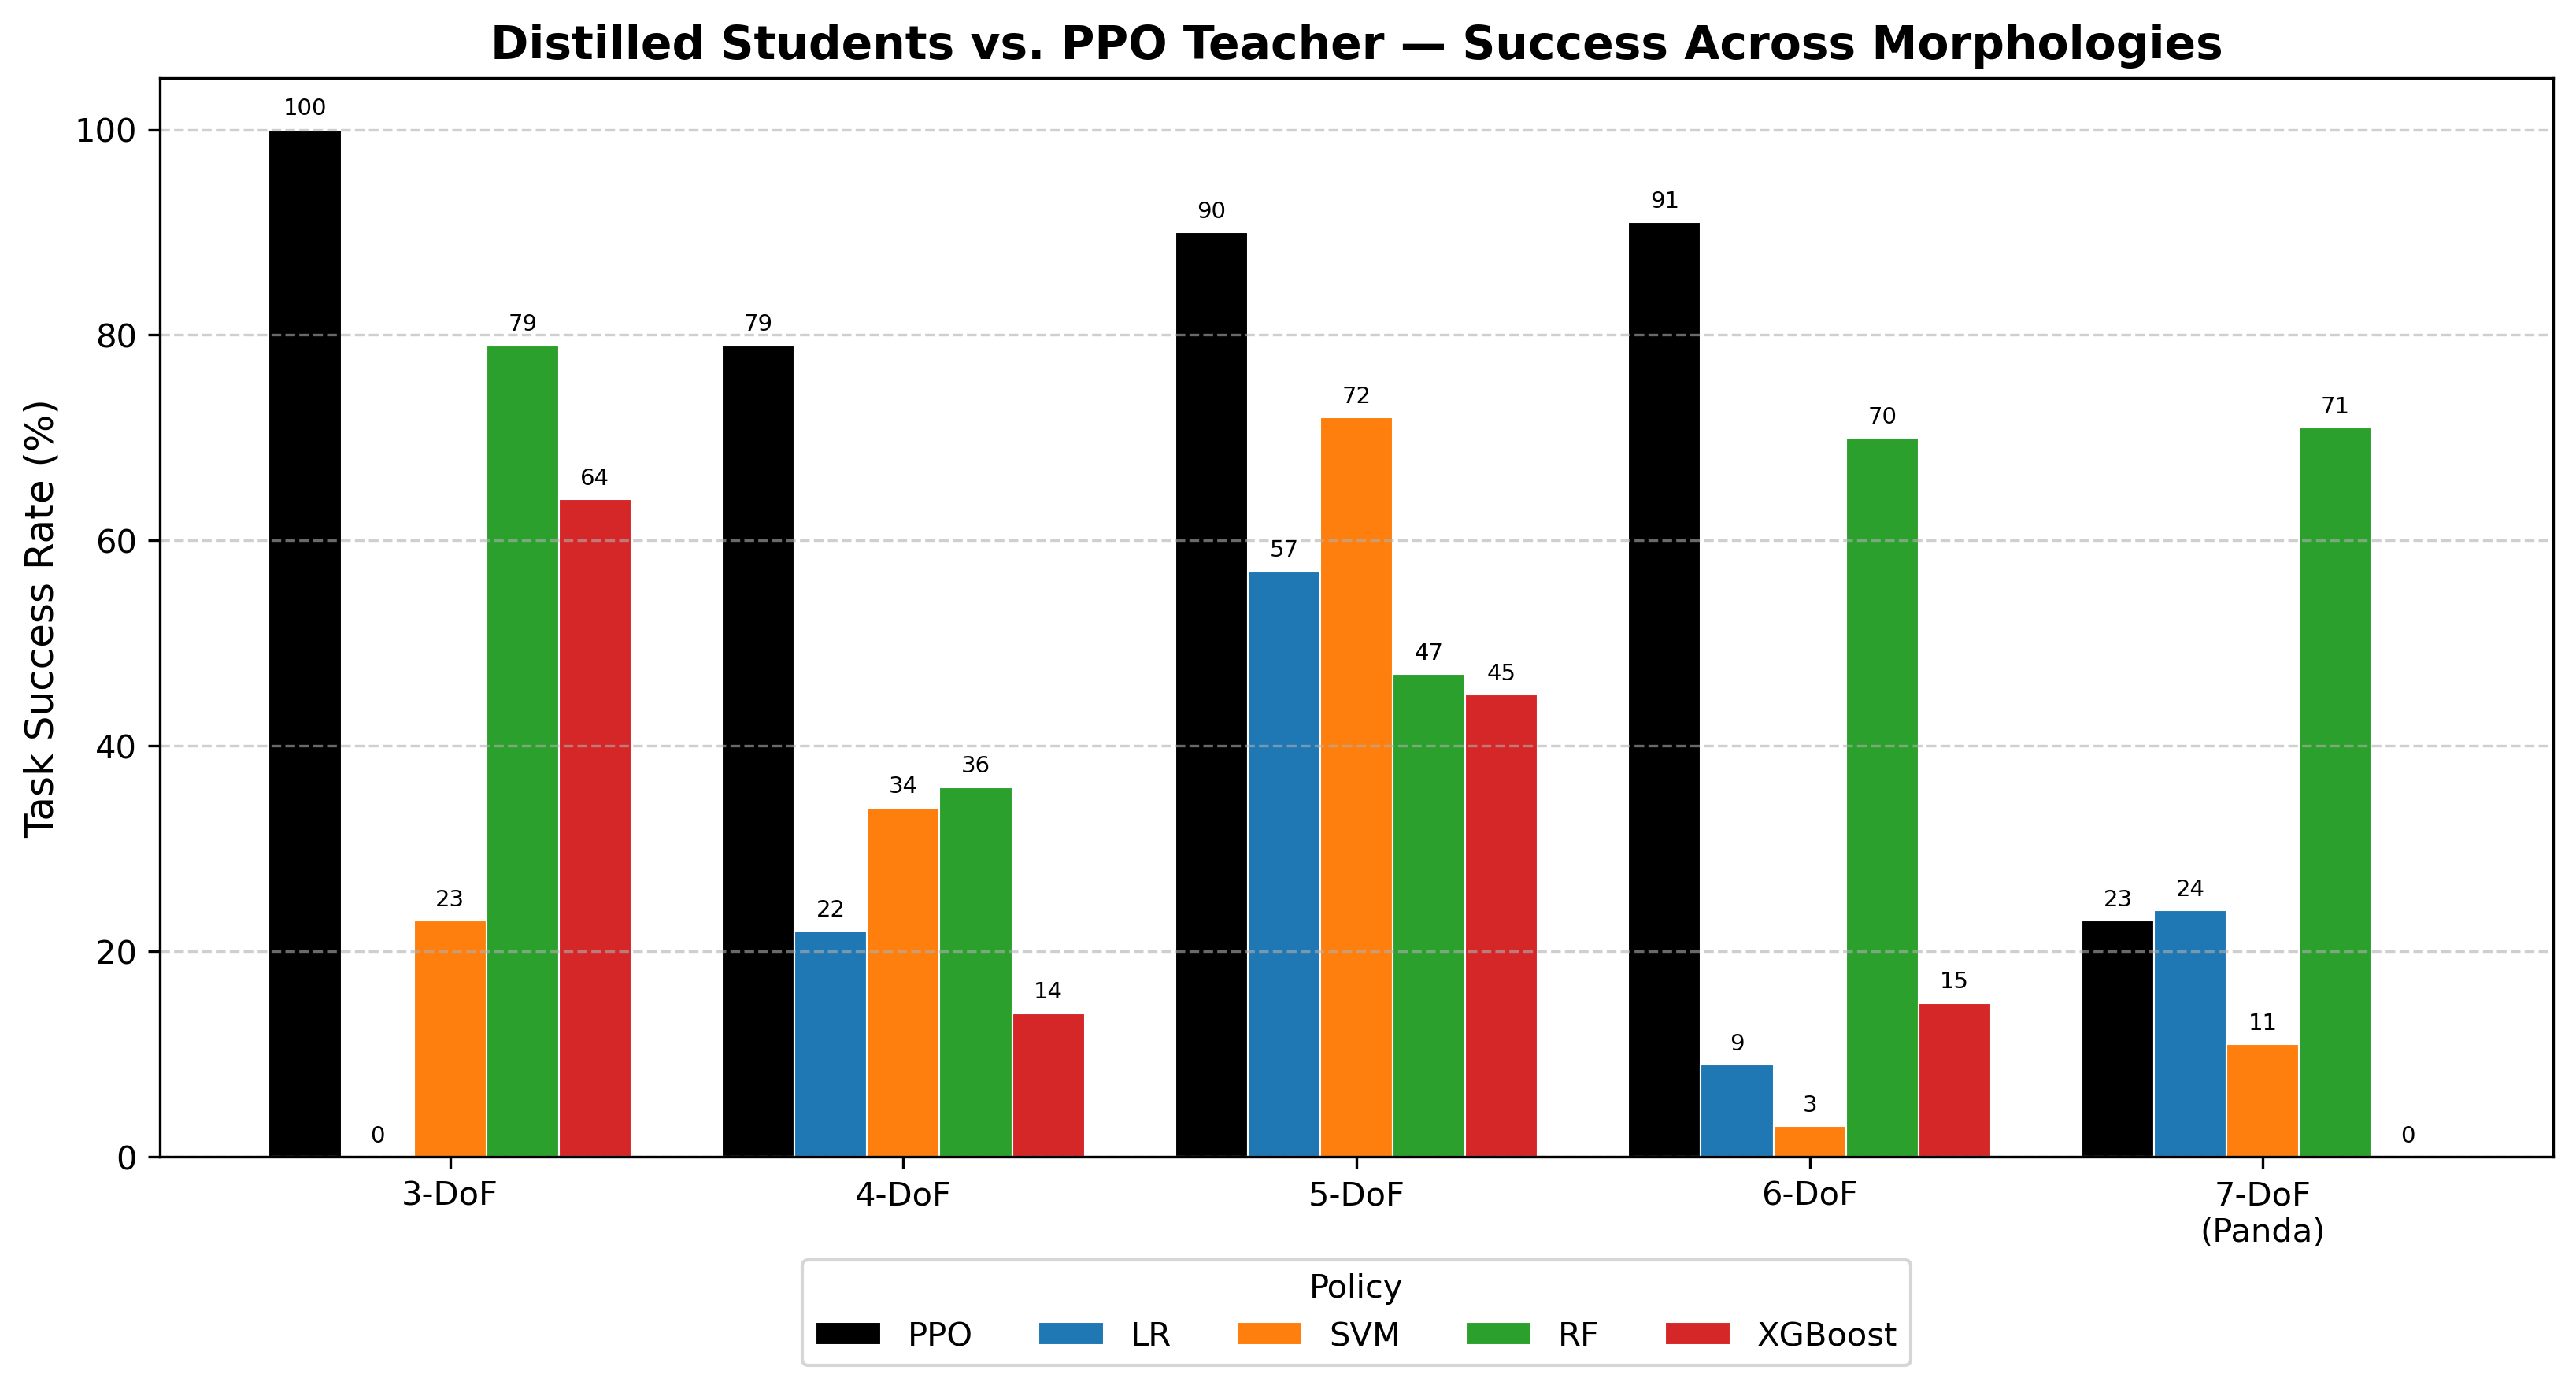
\includegraphics[width=0.92\textwidth]{compare_all_success_bars.png}
\caption{Closed-loop task success of the four distilled students and the PPO
teacher across all five morphologies (100 episodes each, primary run). The
random forest is the most reliable student and surpasses the teacher on the
7-DoF Panda; this gap holds across two teacher checkpoints and six re-trainings,
tracing a saturating teacher--student transfer curve
(see Table~\ref{tab:rf_variance}).}
\label{fig:bars}
\end{figure*}

\subsection{Imitation fidelity}
Table~\ref{tab:r2} reports the held-out $R^2$ of the one-step delta-action
prediction. Fidelity is moderate and remarkably uniform across students
($R^2\!\approx\!0.34$--$0.53$), peaking on the mid-range morphologies and dropping
on the 7-DoF Panda, whose teacher trajectories are the least consistent.
The linear student attains the highest fidelity on four
of the five morphologies (up to $R^2=0.53$), edged out only on the Panda by the
random forest. As the next subsection shows, this offline ranking inverts
in closed loop: one-step regression accuracy is necessary but not sufficient for
control, because error is scored independently per step whereas a deployed policy
must remain stable over an entire episode.

\begin{table}[t]
\centering
\caption{Distillation fidelity ($R^2$ of delta-action prediction, held-out test
split). Best model per morphology in \textbf{bold}.}
\label{tab:r2}
\begin{tabular}{lccccc}
\toprule
\textbf{Model} & \textbf{3-DoF} & \textbf{4-DoF} & \textbf{5-DoF} & \textbf{6-DoF} & \textbf{7-DoF} \\
\midrule
LR      & \textbf{0.504} & \textbf{0.526} & \textbf{0.530} & \textbf{0.526} & 0.410 \\
SVM     & 0.448 & 0.451 & 0.485 & 0.455 & 0.340 \\
RF      & 0.468 & 0.484 & 0.496 & 0.500 & \textbf{0.418} \\
XGBoost & 0.442 & 0.465 & 0.488 & 0.484 & 0.346 \\
\bottomrule
\end{tabular}
\end{table}

\subsection{Closed-loop task success across morphologies}
Table~\ref{tab:success} and Fig.~\ref{fig:overlay} report task success when each
model is deployed as a controller for $100$ episodes per morphology---the latter
showing the per-step cumulative-success curves (a)--(e) and the success-rate
matrix (f)---while Fig.~\ref{fig:bars} summarizes the same success
rates as grouped bars. Three observations stand out. First, the
random forest is the most robust student, scoring $47$--$79\%$ across all
five morphologies and winning four of the five; on the redundant 7-DoF Panda it
reaches $71\%$ and exceeds the PPO teacher ($23\%$) in the primary run; a
controlled follow-up with two teacher checkpoints and three re-trainings each
confirms that the RF student beats its teacher in all six runs and traces a
concave teacher--student transfer curve---rising steeply for weak teachers
before saturating (Section~\ref{sec:rf_variance})---so that on hard morphologies
a smoothed ensemble can recover task success an under-trained teacher never
reached. Second, the linear and boosted students are competitive on individual
morphologies---LR and SVM reach $57\%$ and $72\%$ on the 5-DoF arm, and XGBoost
$64\%$ on the 3-DoF arm---but degrade sharply on others (LR fails outright at
$0\%$ on the 3-DoF arm; XGBoost at $0\%$ on the Panda), reflecting their
sensitivity to compounding errors when a single mispredicted step pushes the
state off the teacher's distribution. Third, offline fidelity is a poor predictor
of closed-loop success: LR has the highest one-step $R^2$ on most arms
(Table~\ref{tab:r2}) yet the worst closed-loop reliability---failing
entirely ($0\%$) on the 3-DoF arm---because its unbounded linear extrapolation
amplifies small errors once the state drifts off the teacher's manifold, whereas
the bounded, averaged outputs of the random forest stay stable. This is why we
evaluate every student directly in closed loop.

\begin{table}[t]
\centering
\caption{Closed-loop task success rate (\%), 100 episodes per cell, seed 42.
Teacher under its native \emph{stochastic} policy; students deterministic. Best
\emph{student} per morphology in \textbf{bold}. Under \emph{greedy} evaluation
the 7-DoF teacher's $23\%$ falls to $1\%$ (Table~\ref{tab:rf_variance}).}
\label{tab:success}
\begin{tabular}{lccccc}
\toprule
\textbf{Model} & \textbf{3-DoF} & \textbf{4-DoF} & \textbf{5-DoF} & \textbf{6-DoF} & \textbf{7-DoF} \\
\midrule
PPO (teacher) & 100 & 79 & 90 & 91 & 23 \\
\midrule
LR            & 0  & 22 & 57 & 9  & 24 \\
SVM           & 23 & 34 & \textbf{72} & 3  & 11 \\
RF            & \textbf{79} & \textbf{36} & 47 & \textbf{70} & \textbf{71} \\
XGBoost       & 64 & 14 & 45 & 15 & 0  \\
\bottomrule
\end{tabular}
\end{table}

\subsection{The teacher--student transfer curve}
\label{sec:rf_variance}

The most important finding of this study concerns \emph{how} the distilled
student's competence relates to its teacher's. To map this relationship on the
7-DoF Panda we evaluated RF students against teachers of differing skill, using
two teacher checkpoints and three independent RF re-trainings each (100 episodes
per run, seeds $\{42,0,123\}$). The first teacher (seed~42, $10{,}000$ training
episodes) solves $23\%$ of test episodes; the second (seed~0, $1{,}000$
episodes) is deliberately under-trained and solves only $4\%$. Students are
distilled \emph{only} from each teacher's successful rollouts.
Table~\ref{tab:rf_variance} reports all six runs, ordered by teacher competence.

\begin{table}[t]
\centering
\caption{Teacher--student transfer on the 7-DoF Panda (100 episodes each). The
teacher is shown under both its test-time \emph{sampled} policy and a
\emph{greedy} (mean-action) re-evaluation; the deterministic RF student is
listed by its three runs and mean. The teacher's sampled success is
\emph{noise-borrowed}: under greedy evaluation it collapses to $0$--$1\%$, while
the deterministic student retains $27$--$55\%$.}
\label{tab:rf_variance}
{\setlength{\tabcolsep}{3.5pt}\footnotesize
\begin{tabular}{lcccc}
\toprule
\textbf{Teacher} & \textbf{Teacher} & \textbf{Teacher} & \textbf{RF runs} & \textbf{RF mean} \\
\textbf{checkpoint} & \textbf{sampled} & \textbf{greedy} & \textbf{(\%)} & \textbf{(\%)} \\
\midrule
none\textsuperscript{$\dagger$}  & 0\%  & 0\% & ---          & 0 \\
weak (s0, 1k ep)                 & 4\%  & 0\% & 33,\,14,\,34 & 27.0 \\
stronger (s42, 10k ep)           & 23\% & 1\% & 71,\,43,\,52 & 55.3 \\
\bottomrule
\end{tabular}}

\vspace{2pt}
{\footnotesize $\dagger$ A teacher that never succeeds yields no distillation
data, so the student is $0\%$ by construction---a fixed anchor for the curve.}
\end{table}

\begin{figure}[t]
\centering
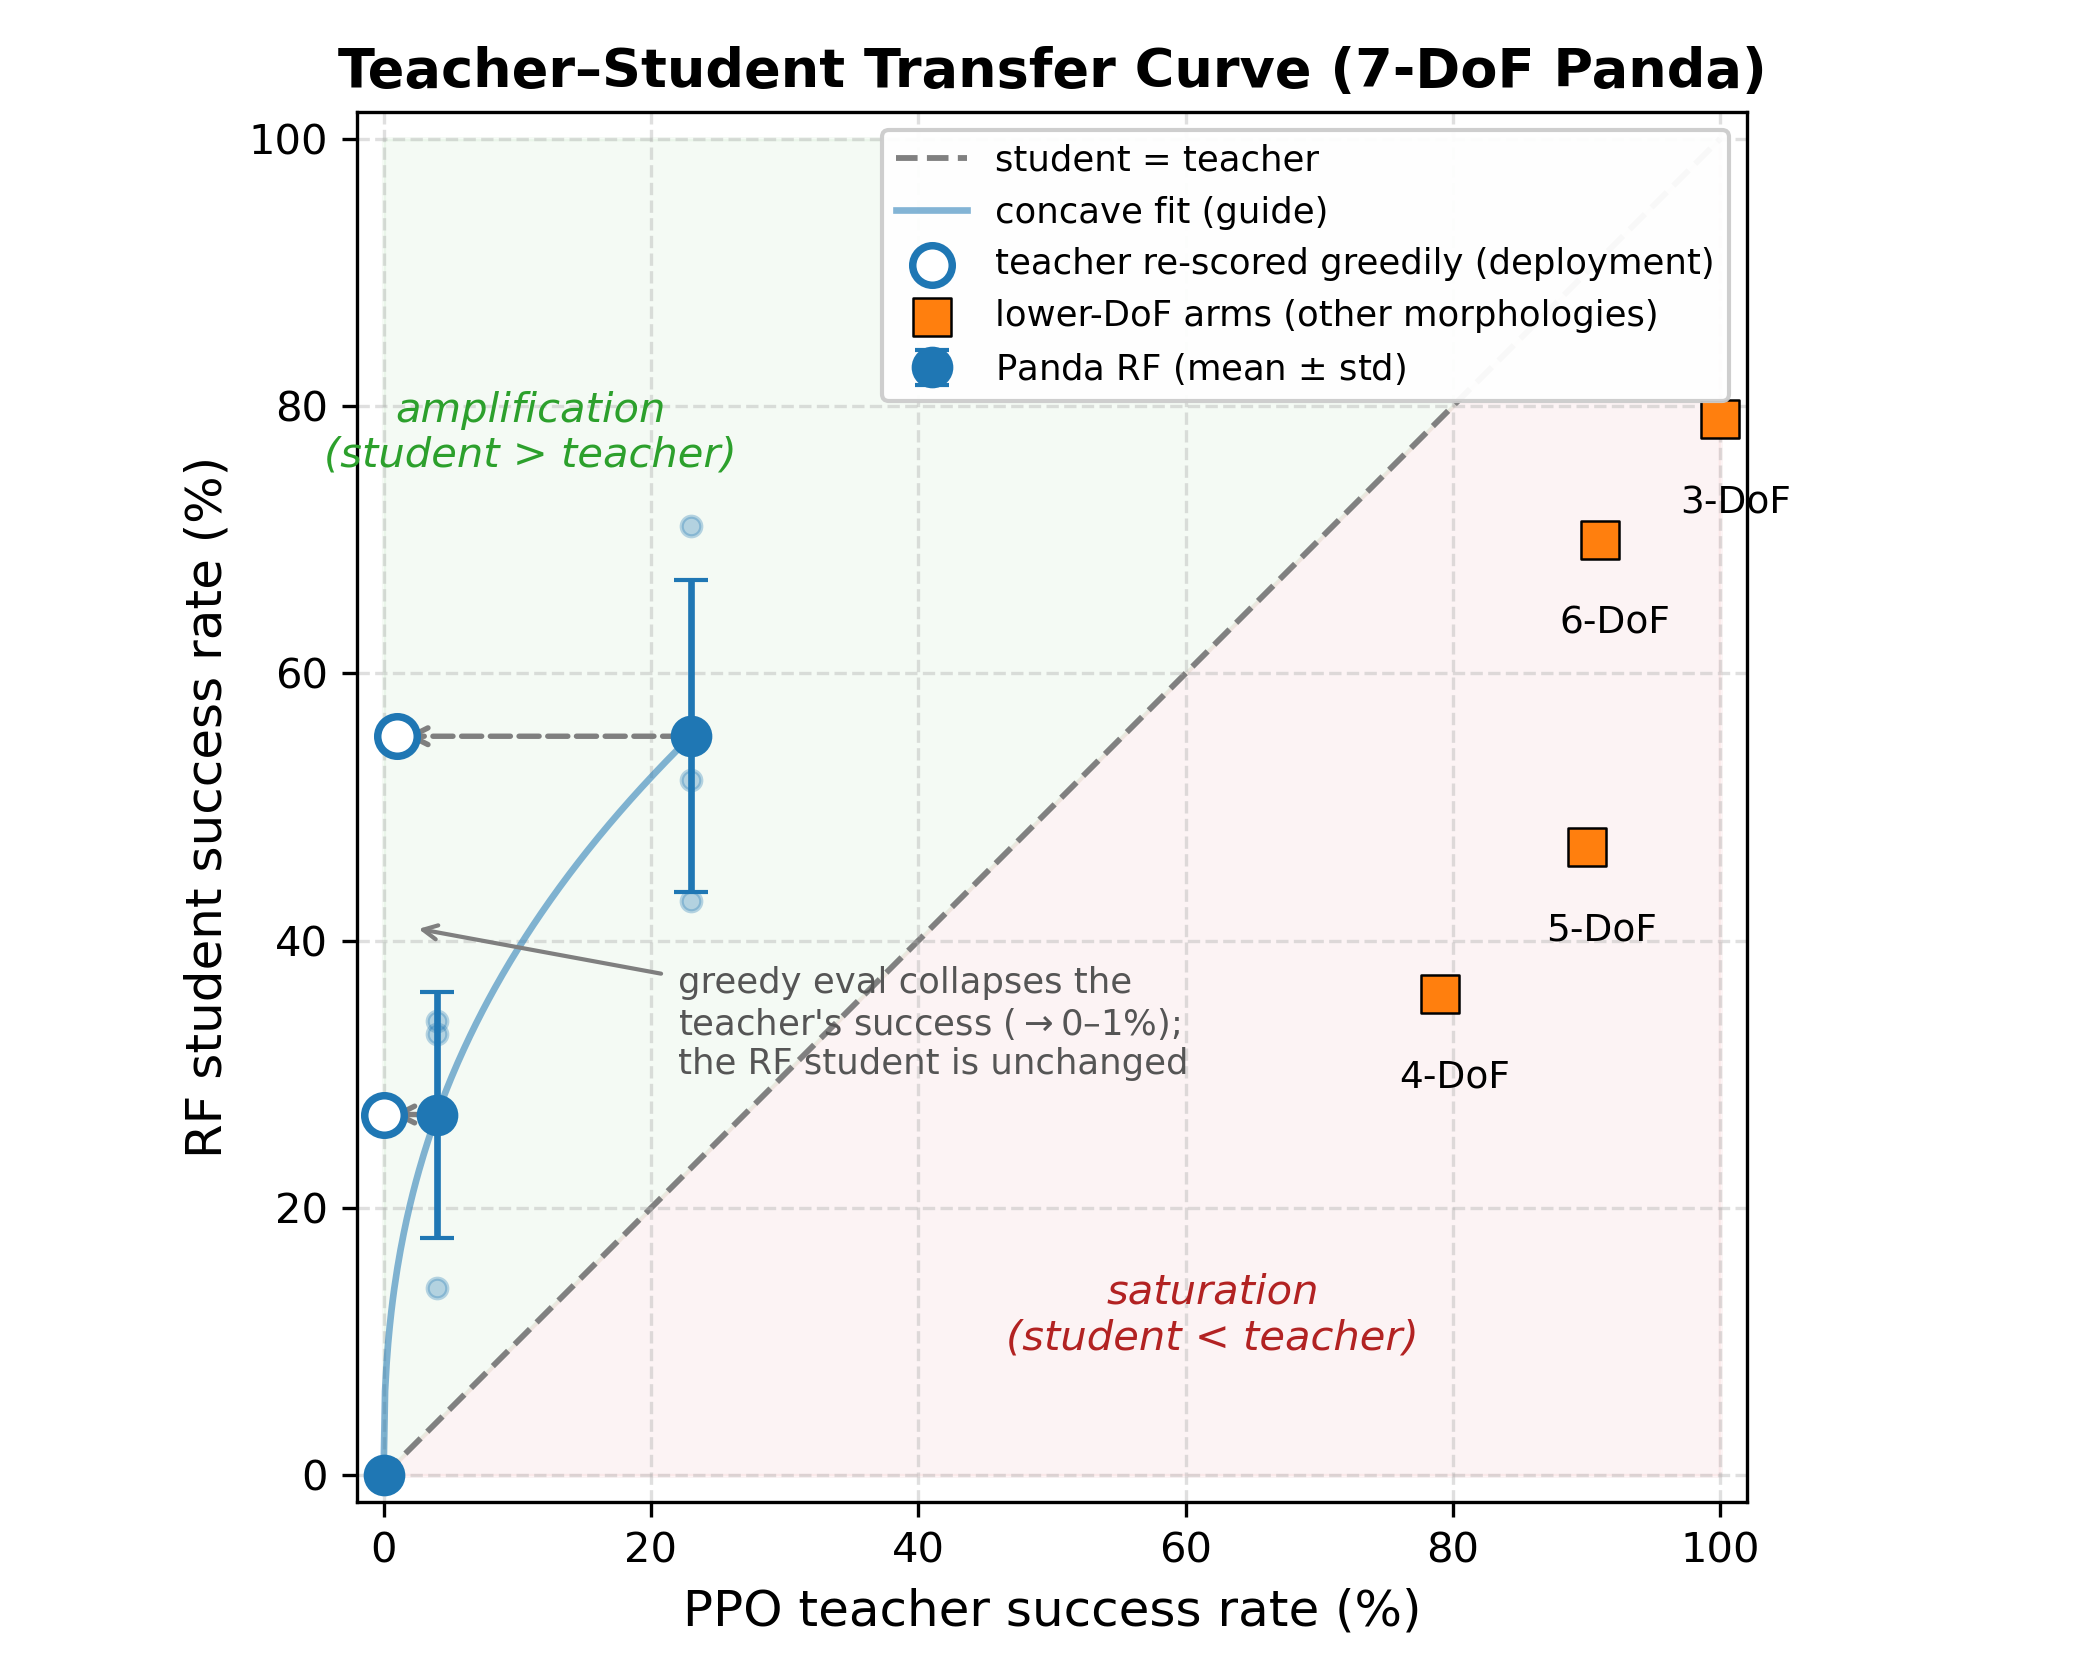
\includegraphics[width=\columnwidth]{transfer_curve.png}
\caption{Teacher--student transfer on the 7-DoF Panda. The deterministic RF
student's success (faint dots: individual runs; filled circles: mean $\pm$std) is
plotted against PPO teacher success, anchored at the trivial $(0,0)$ point. Open
circles re-score the \emph{same} teachers \emph{greedily} (mean action): their
success collapses to $0$--$1\%$ (dashed arrows) while the student is unchanged,
showing the teacher's sampled success is exploration-noise-borrowed. The student
sits well above the student\,$=$\,teacher diagonal here (amplification region);
on the lower-DoF arms (squares; other morphologies), whose teachers are genuinely
competent \emph{despite} the same action noise, the students fall below the
diagonal (saturation region).}
\label{fig:transfer}
\end{figure}

Read together with the trivial anchor at the origin, the three points trace a
\emph{concave, saturating} transfer curve rather than a proportional one
(Fig.~\ref{fig:transfer}).
Student success rises \emph{steeply} where the teacher is weak: lifting the
teacher from $0\%$ to merely $4\%$ already carries the RF student to $27\%$, and
$4\%\to23\%$ carries it to $55\%$. The \emph{marginal} return, however, falls
off sharply---roughly $7$ student points per teacher point near the origin
versus under $1.5$ thereafter---so the curve bends over as the teacher improves.
On the easier low-DoF arms, by contrast, a genuinely competent teacher
($90$--$100\%$) is \emph{no longer} surpassed by its student (RF $47$--$79\%$,
Table~\ref{tab:success}): the student leads against the weak 7-DoF teacher but
trails the strong low-DoF ones. (Run-to-run spread, e.g.\ $14$--$34\%$ at the
$4\%$ teacher, reflects Gazebo stochasticity but never reverses the ordering.)
The next paragraph traces this split to the teacher's reliance on exploration
noise.

A deterministic re-evaluation exposes the mechanism behind this curve. The PPO
actor carries a large \emph{learned} action noise---standard deviation
$\approx\!1.0$ on the normalized $[-1,1]$ action range, and nearly identical
($0.99$--$1.24$) across all five morphologies---and it \emph{samples} that noise
at every test step. Evaluated greedily instead, taking the mean action as one
would at deployment, the Panda teacher collapses: from $4\%$ to $0\%$ (weak
checkpoint) and from $23\%$ to $1\%$ (strong checkpoint), see
Table~\ref{tab:rf_variance}. Its apparent competence is almost entirely
\emph{noise-borrowed}---the policy never distilled the task into a usable
deterministic controller and instead relies on its own exploration noise to
stumble onto success. The RF student is inherently deterministic, yet retains
$27$--$55\%$. Distillation thus does more than compress the teacher: by averaging
the rare successful (noise-driven) rollouts into a smooth, repeatable policy, it
\emph{recovers a deployable controller the teacher does not itself possess}.

The same view explains why the advantage is confined to the redundant 7-DoF arm.
The identical $\approx\!1.0$ noise is present on the low-DoF arms, yet their
teachers still solve $79$--$100\%$ of episodes. Noise-borrowed success caps out
at the low rates we measure on the Panda ($\le 23\%$); a teacher that succeeds
$90\%$ of the time \emph{under} that noise must therefore have a genuinely
competent mean policy. Against such a teacher a one-shot imitator cannot improve
and settles below it. The teacher--student curve consequently reflects a
transition in the \emph{teacher}: from genuinely solved (low-DoF, where the
student trails a truly competent policy) to only-noise-solved (7-DoF, where the
student supplies the deployable policy the teacher lacks). Characterizing this
transition across the full competence range is an important direction for future
work.

\subsection{Model footprint and inference latency}
Table~\ref{tab:footprint} reports measured footprint and single-step latency.
This contrast is the central deployment finding. The linear student
is \(1.4\)--\(4.7\)~kB (roughly \(30\)--\(100\times\) smaller than the
\(\approx\!150\)~kB teacher network) and predicts in \(\approx\!0.2\)~ms,
faster than the teacher's own forward pass. XGBoost and the SVM occupy a
few megabytes and run in single-digit-to-low milliseconds. The random forest,
despite its fidelity advantage, is \(30\)--\(127\)~MB and \(110\)--\(251\)~ms per
step, one to three orders of magnitude slower than every alternative and beyond a
typical real-time control budget.

\begin{table}[t]
\centering
\caption{Measured footprint and CPU inference latency (range over 3--7~DoF).}
\label{tab:footprint}
\begin{tabular}{lcc}
\toprule
\textbf{Model} & \textbf{Footprint} & \textbf{Latency (ms/step)} \\
\midrule
LR              & 1.4--4.7~kB   & 0.19--0.21 \\
SVM             & 2.0--7.2~MB   & 2.1--5.0 \\
RF              & 30--127~MB    & 110--251 \\
XGBoost         & 2.1--3.9~MB   & 4.5--8.4 \\
\midrule
PPO (teacher)   & $\approx$150~kB & 0.74--0.84 \\
\bottomrule
\end{tabular}
\end{table}

\subsection{Discussion}
The results expose a three-way tension between control performance, robustness,
and efficiency. On control performance, the random forest clearly leads
(Table~\ref{tab:success}): as a high-capacity ensemble it absorbs the teacher's
nonlinear mapping and, by averaging many trees, produces smooth low-variance
actions that compound gracefully in closed loop---to the point of beating an
under-trained teacher on the Panda. On efficiency, the ordering inverts
(Table~\ref{tab:footprint}): LR is the smallest and fastest model, even relative
to the neural teacher, while the random forest is prohibitively heavy at
$30$--$127$~MB and $110$--$251$~ms per step. The linear and boosted students sit
in between but are inconsistent---strong on some morphologies, failing on
others---because a single large one-step error can drive the system off the
teacher's data manifold, after which subsequent predictions degrade.

A central finding concerns the relationship between teacher and student
competence. On the 7-DoF Panda the random forest consistently outperforms its
teacher across two checkpoints---three re-trainings each, six runs---reaching
$27\%$ from a $4\%$ teacher and $55\%$ from a $23\%$ one
(Table~\ref{tab:rf_variance}). A deterministic re-evaluation explains why: the
PPO actor samples a large learned action noise ($\mathrm{std}\!\approx\!1.0$,
near-identical across morphologies) at test time, and the Panda teacher's
success is largely an artifact of that noise---under greedy evaluation it
collapses to $0$--$1\%$, whereas the deterministic student keeps $27$--$55\%$.
On this hard, redundant arm the teacher never learned a usable deterministic
policy; distillation, by averaging its rare successful rollouts into a smooth
repeatable controller, \emph{recovers a deployable policy the teacher does not
itself possess}. The advantage is confined to the 7-DoF arm precisely because
noise-borrowed success caps out at low rates: the low-DoF teachers solve
$79$--$100\%$ \emph{despite} the same noise, so their mean policies are genuinely
competent and a one-shot imitator cannot exceed them. Characterizing this
genuinely-solved$\rightarrow$noise-solved transition across the full competence
range is an important direction for future work.

The practical recommendation is therefore deployment-dependent. Where compute
permits, the random forest gives the best and most uniform task success and is the
safest default. For the tight memory and latency budgets typical of MSME edge
controllers, the linear or boosted students are attractive \emph{if} validated
per morphology, since their closed-loop reliability does not track offline
regression error: a model can minimize one-step error yet still drift over a full
episode, which is why end-to-end closed-loop evaluation---not $R^2$ alone---is the
decisive metric.

%==============================================================================
\section{Limitations and Future Work}
%==============================================================================
The students imitate a fixed teacher on successful trajectories only; they inherit
its behavior and its biases and are not expected to recover from states the
teacher never visited. The target object spawns at a fixed location, so learned
policies may not generalize across the workspace. The derivative features depend
on a time step that is approximated at deployment. The policy-recovery effect is
established on a single hard morphology and three teacher-competence points;
mapping the full genuinely-solved$\rightarrow$noise-solved transition would
require teacher checkpoints spanning the competence range. We report teacher
success under its native stochastic policy, with greedy (deployment-mode)
evaluation given separately for the 7-DoF arm; a uniform greedy comparison across
all morphologies would further tighten the picture. Future work includes
DAgger-style on-policy data aggregation to cover off-distribution states, domain
randomization of object placement and physics for robustness, distillation
directly to torque commands, and validation on physical hardware to assess the
real latency and footprint benefits under actuator dynamics.

%==============================================================================
\section{Conclusion}
%==============================================================================
We presented a pipeline that distills a morphology-agnostic PPO manipulation
policy into compact classical models---LR, SVM, RF, and XGBoost---trained on
teacher rollouts to predict delta-actions and deployed directly as closed-loop
controllers across 3--7~DoF arms. Footprint and latency reveal a clear
trade-off: the linear student is dramatically smaller and faster than the neural
teacher, while the random forest gives the most reliable control at a heavy
runtime cost---and closed-loop success, not one-step regression accuracy, is what
separates the students. Most notably, on the redundant 7-DoF arm---where the PPO
teacher's success proves to be largely an artefact of its exploration noise and
nearly vanishes under greedy evaluation---the deterministic random-forest student
recovers a deployable controller the teacher does not itself possess. Distillation
thus offers more than compression: a route to deployable, inspectable manipulation
controllers that can, on hard morphologies, even surpass the policy they are
distilled from, with the appropriate student selected per the target platform's
accuracy and efficiency constraints.

%==============================================================================
\begin{thebibliography}{00}

\bibitem{hinton} G.~Hinton, O.~Vinyals, and J.~Dean, ``Distilling the knowledge
in a neural network,'' \emph{arXiv:1503.02531}, 2015.

\bibitem{rusu} A.~A.~Rusu \emph{et al.}, ``Policy distillation,'' in
\emph{Proc. Int. Conf. Learn. Represent. (ICLR)}, 2016.

\bibitem{schulman} J.~Schulman, F.~Wolski, P.~Dhariwal, A.~Radford, and
O.~Klimov, ``Proximal policy optimization algorithms,''
\emph{arXiv:1707.06347}, 2017.

\bibitem{breiman} L.~Breiman, ``Random forests,'' \emph{Machine Learning},
vol.~45, no.~1, pp.~5--32, 2001.

\bibitem{xgboost} T.~Chen and C.~Guestrin, ``XGBoost: A scalable tree boosting
system,'' in \emph{Proc. ACM SIGKDD}, 2016, pp.~785--794.

\bibitem{kober} J.~Kober, J.~A.~Bagnell, and J.~Peters, ``Reinforcement learning
in robotics: A survey,'' \emph{Int. J. Robotics Research}, vol.~32, no.~11,
pp.~1238--1274, 2013.

\bibitem{lobbezoo_survey} A.~Lobbezoo, Y.~Qian, and H.-J.~Kwon, ``Reinforcement
learning for pick and place operations in robotics: A survey,'' \emph{Robotics},
vol.~10, no.~3, p.~105, 2021.

\bibitem{shahid} A.~A.~Shahid, L.~Roveda, D.~Piga, and F.~Braghin, ``Learning
continuous control actions for robotic grasping with reinforcement learning,'' in
\emph{Proc. IEEE SMC}, 2020, pp.~1--6.

\bibitem{elguea} \'I.~Elguea-Aguinaco \emph{et al.}, ``A review on reinforcement
learning for contact-rich robotic manipulation tasks,'' \emph{Robotics and
Computer-Integrated Manufacturing}, vol.~81, p.~102517, 2023.

\bibitem{panda_gym} Q.~Gallou\'edec, N.~Cazin, E.~Dellandr\'ea, and L.~Chen,
``panda-gym: Open-source goal-conditioned environments for robotic learning,'' in
\emph{4th Robot Learning Workshop, NeurIPS}, 2021.

\bibitem{luo} Y.~Luo, Y.~Dong, L.~Zhang, Y.~Wang, and F.~Sun, ``Balance between
efficient and effective learning: Dense2Sparse reward shaping for robot
manipulation with environment uncertainty,'' \emph{arXiv:2003.02740}, 2020.

\end{thebibliography}

\end{document}
